% !TeX root = ../main.tex

\chapter{IPv6源地址验证技术增强方案}
\label{IPv6_Security}

  \section{本章引言}
  \label{IPv6_Security:introduction}
  网络中的源地址真实是实现用户身份识别与溯源的前提。只有保证了源地址的真实,并将真实的IP地址与用户身份正确地进行绑定,才能够实现通过分析攻击流量定位源IP地址、根据源IP地址溯源攻击者实体的功能。
  按照源地址验证体系结构SAVA的划分层次,接入子网、自治域内和自治域间均可能发生源地址的伪造情况。接入子网作为最靠近用户的层级,其能够提供最细粒度的源地址伪造过滤机制,具有最为基础且深刻的作用。理想情况下,当所有自治域内所有接入子网均能确保不发生子网内的源地址伪造时,自治域内与自治域间的源地址伪造问题便已不复存在。但是,在实际的网络中,自治域间不属于一个管理域,其安全技术的选择与部署包含着自身的利益考虑,不可能进行整体的协调,因此仍需要SAVA中各级机制互相配合以在设备粒度、子网粒度与自治域粒度三个层次预防IPv6源地址的伪造。

  对于基于IPv6地址追溯用户身份的用户身份识别与溯源系统而言,由其提供网络接入服务的用户子网必须要求设备粒度的源地址真实性验证,以确保IPv6源地址可以准确地关联到需要对报文负责的用户实体。自治域内与自治域间也需要提供预防系统部署子网IPv6地址遭到伪造的机制,以保证使用用户身份识别与溯源系统接入的用户不会因为被其他子网或其他自治域的恶意用户假冒地址而被错误追责。

  目前,接入子网的源地址验证技术SAVI已基本全部被标准化,但其在网络中实际部署应用时仍可能面临厂商设备尚未支持或版本过旧、替换或升级成本较高等问题,对用户身份识别与溯源系统的部署使用造成一定阻碍。同时,源地址验证作为一项解决网络安全问题的基础技术,其本身也可能成为恶意攻击者的攻击目标。本章首先分析SAVI技术部署在实际网络中面临的困境,利用传统设备普遍支持的VLAN功能,提出在已有网络环境中以较小代价支持接入子网源地址伪造预防的增强方案,然后针对自治域间源地址验证这一层次,研究其目前一类基于端到端验证思路的主流方案所共有的安全隐患,以其中典型的SMA为例,提出了基于区块链的增强方案设计,并进行了实现与测试,为端到端类域间源地址验证技术提供了统一的安全性改进思路。

  本章内容组织如下:第\ref{IPv6_Security:access}节分析为用户身份识别与溯源系统提供基础支持的SAVI技术在部署时的要求与困境,并提出了在难以进行接入交换机SAVI全支持的网络中实现接入子网内IPv6源地址防伪造的增强方案设计;第\ref{IPv6_Security:interas}节以SMA方案为例对端到端验证类思想的域间源地址验证技术的安全性进行分析,针对SMA方案中REG中心化设计的问题,研究了其联盟注册系统的区块链设计方案RegChain,并在以太坊平台上进行了实现与验证;第\ref{IPv6_Security:summary}节对本章内容进行总结。

  \section{接入子网源地址验证技术增强方案}
  \label{IPv6_Security:access} 

    \subsection{SAVI技术的部署与分析}
    \label{IPv6_Security:access:deploy}

    为了发挥SAVI技术的作用,子网内部署SAVI的设备必须形成一个安全边界,以确保所有设备发出的数据报文在通过子网网关转发前必定经过一台SAVI设备对源地址进行检查。SAVI设备形成的安全边界越靠近用户设备,则能够实现的源地址过滤粒度越精细。如\ref{survey:sava:access:bound}节所述,当有线网络中SAVI安全边界某一个端口下不止一台用户设备时,由于用户设备均对应同一个绑定锚,SAVI设备难以根据IP地址与绑定锚的绑定关系区分来自不同设备的流量,因而难以防止设备之间互相伪造源地址。

    因此,要实现接入子网内不发生源地址伪造,必须由直接连接用户、提供接入的接入交换机或无线接入点部署SAVI、实施伪造源地址报文的过滤:
    \begin{enumerate}[1{)}]
      \item \textbf{无线网络}:在基于无线控制器的集中控制组网方式下,只需要在AC上对接入子网配置SAVI的启用,并根据子网内地址配置方式启用DHCPv6 Snooping或ND Snooping即可。目前华为、新华三等几大设备厂商生产的AP与AC均已支持无线SAVI技术。
      \item \textbf{有线网络}:所有包含接入子网端口的接入交换机全部启用SAVI,确保安全边界端口下连仅有一台用户设备。对于用户在网络管理员所能控制的交换机端口下仍私接交换机的情形,我们认为这是用户的非法行为,发生其下多台设备之间的互相伪造最终被判定由同一用户负责是符合情理的处理结果。
    \end{enumerate}

    但是,在推动各所高校进行接入子网源地址验证技术的部署时,SAVI技术很难做到上述理想情况的部署。对于无线网络,由于不存在链路实体,用户设备通过射频信号与AP进行链路建立和通信,因此即使网络环境中存在版本过旧而不支持SAVI技术的AP,我们仍可以简单地选择不在其上开设进行源地址验证的接入子网的信号。而对于有线环境,情况则较为复杂,网络中接入交换机数量众多,品牌、型号各异,极有可能存在部分接入交换机支持SAVI而另一部分不支持的情况,对于地理位置相近、身份类别相同的用户,由于其上连的接入交换机对SAVI的支持情况不同而为其划分不同的子网、提供不同的接入服务,容易造成用户不良的体验,因此仍需提出在难以将接入交换机全部替换以支持SAVI的情况下如何对非SAVI接入交换机接入用户同样进行IPv6源地址验证的增强方案。

    \subsection{基于VLAN划分的SAVI部署增强方案}
    \label{IPv6_Security:access:enhance}
    尽管将接入交换机全部替换为支持SAVI的设备可能成本较高,但为了部署SAVI技术,必须要在网络中形成安全边界,因此对于非SAVI交换机,其上连至网关的链路中必须有一台交换机支持SAVI。对于二层交换机多级连接的情况,尽量替换靠近用户设备层级的交换机,在最坏情况下,汇聚交换机下所有交换机均不支持SAVI,则汇聚交换机必须支持SAVI。在构成了SAVI安全边界的前提下,若接入子网中存在不支持SAVI的接入交换机,我们可以通过配合特殊的VLAN划分方法实现整个接入子网内的源地址防伪造方案,如图\ref{fig:SAVI_enhance}所示。

    \begin{figure}[ht]
      \centering
      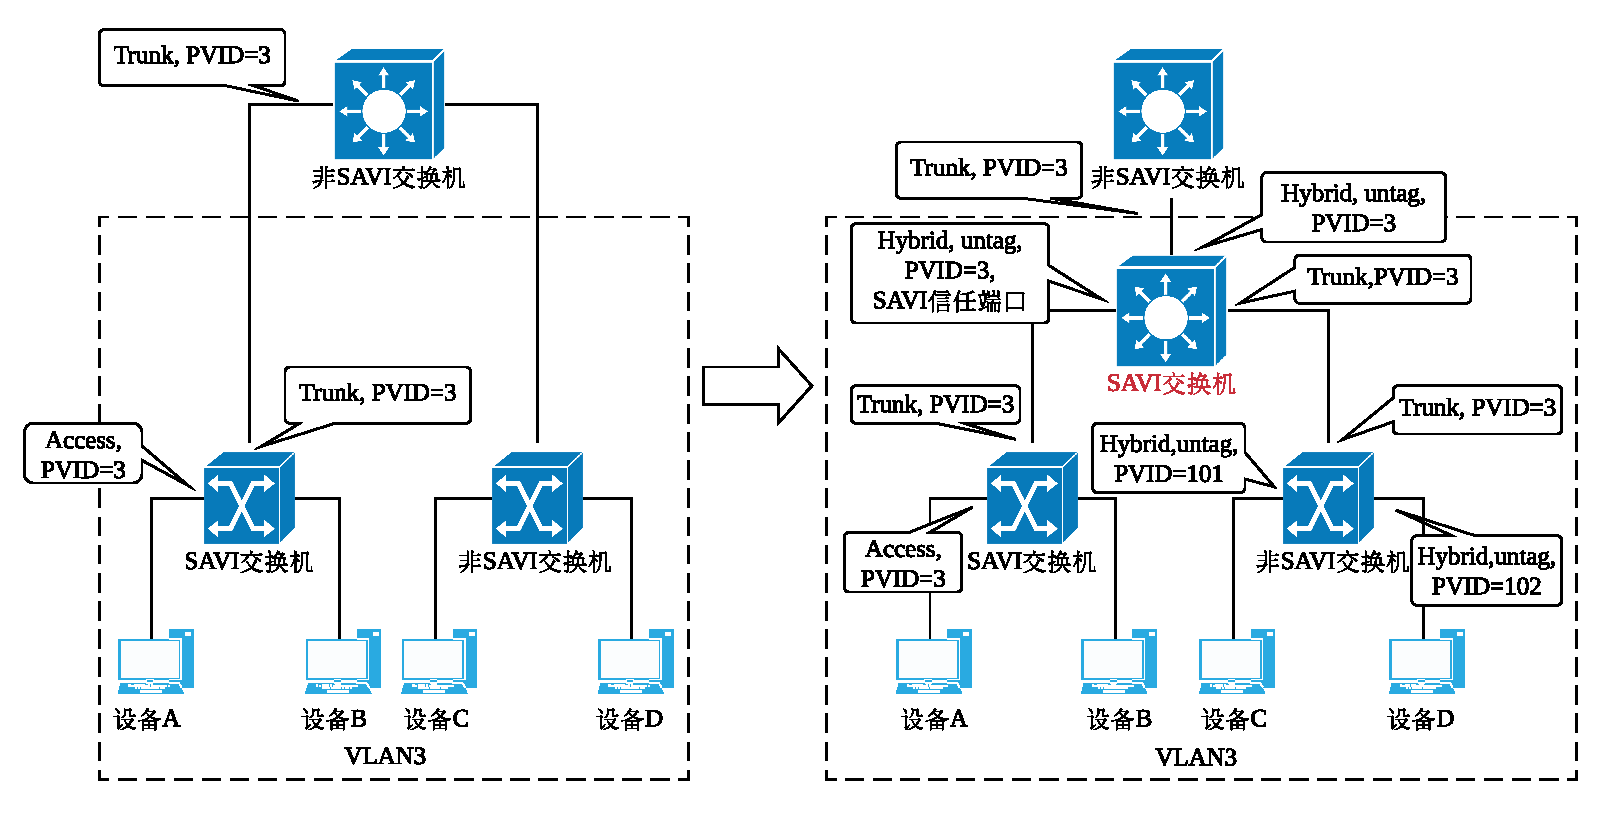
\includegraphics[width=\textwidth]{SAVI_enhance.pdf}
      \caption{基于VLAN划分的SAVI部署增强方案示意}
      \label{fig:SAVI_enhance}
    \end{figure}

    图\ref{fig:SAVI_enhance}左侧为一个有线网络典型的组网拓扑,子网网关位于汇聚交换机上,汇聚交换机下连接有多台接入交换机,接入交换机的端口将直连用户有线设备,提供有线网络的接入服务。一般而言,汇聚交换机数量较少,比如在一栋楼宇中部署一台,而接入交换机则数量众多,一个房间可能就部署不止一台。左图所示接入交换机中,部分不支持SAVI技术,将其全部替换为支持SAVI的设备需要较大的费用开销与网络迁移工程。显然,对于左侧的VLAN 3这一子网,由于SAVI设备没有构成安全边界,仅有设备A、B不可伪造源地址,设备C与D不仅可以互相伪造对方的地址,也可以伪造设备A与B的源地址以及任意其他IPv6地址,无法提供接入子网IPv6源地址的真实性保障。

    如\ref{survey:sava:access:listen}节所述,在有线网络中,SAVI会以源地址与VLAN为索引建立绑定表项,因此图\ref{fig:SAVI_enhance}右侧结合VLAN信息提出IPv6源地址验证的增强方案。首先,虽然无法将所有不支持SAVI的接入交换机进行替换,但我们在接入层与汇聚交换机之间新增一台SAVI交换机(红字标注),即可构成SAVI所要求的安全边界。此时,尽管仍然无法防止设备C与设备D之间互相的源地址伪造,但已大大缩减了它们所能伪造的地址范围,从整个IPv6地址空间缩小到了SAVI交换机下接入的各个设备的源地址,当然也保障了设备A与B的源地址不会被同子网内的其他设备所伪造。然后,我们通过图示的VLAN划分手段,来防止设备C与D之间的互相伪造问题。首先以设备C为例,考察其上行流量与下行流量所携带的VLAN标签:
    \begin{itemize}
      \item \textbf{上行流量}:由设备C发出的报文到达接入交换机后,根据Hybrid端口的检查规则,由于其不带有VLAN标签,交换机向其中加入101号VLAN标签;在允许VLAN 101经过的上连Trunk口,经过Trunk口检查规则,与其PVID=3不匹配,因此保持VLAN号101向上转发;到达SAVI交换机的下连Trunk口时,与其PVID=3不匹配,仍保持VLAN号101;由上连至原汇聚交换机的Hybrid口发出时,由于该端口配置了untag,因此VLAN号101被剥离,在到达汇聚交换机的PVID=3的Trunk口时被重新打上VLAN号为3的标签,进行后续转发。
      \item \textbf{下行流量}:由汇聚交换机向下转发的流量在下连的Trunk口被剥离VLAN号3的标签,在进入SAVI交换机的Hybrid口时被重新加上3号VLAN的标签;在转发至接入交换机时同样在下连的Trunk口剥离3号VLAN标签,由接入交换机的上连Trunk口加入3号VLAN标签;在转发至设备时,设备C所连接的Hybrid端口允许3号VLAN报文通过,并根据untag的配置将其VLAN号剥离后进行转发。
    \end{itemize}

    可见,由设备C发出的报文在到达SAVI交换机时将携带101号VLAN标签,而在到达子网网关时将携带3号VLAN的标签,其内部的101号VLAN对于接入子网外部而言不可见。对于由汇聚交换机下发的报文,其3号VLAN标签将在最终到达用户设备时被剥离,从而使设备网卡能够正常识别并进行处理。在这种情况下,在新增的设备开启SAVI功能后,设备C与设备D互相之间的源地址伪造也将被避免:
    \begin{enumerate}[1{)}]
      \item 当设备C配置IPv6地址时,新增的SAVI交换机将其IPv6地址、VLAN号101与其下连端口相绑定。同样,设备D配置的IPv6地址也将与VLAN号102、下连同一端口相绑定。
      \item 当设备C伪造设备D的MAC地址与源IP地址向外发送报文时,其报文在经过接入交换机端口后将携带VLAN号101到达SAVI交换机。
      \item SAVI交换机根据SAVI绑定表,检查报文中的IPv6地址、VLAN号、MAC地址与端口号,发现虽然IPv6地址、MAC地址与端口号绑定一致,但VLAN号101与绑定表中IPv6地址所绑定的102号VLAN不匹配,说明该报文为源地址伪造报文,将其丢弃。
    \end{enumerate}
    
    因此,在无法实现接入交换机全部部署SAVI技术的情况下,本文给出了一种结合VLAN实现IPv6源地址验证增强的方案,防止了SAVI安全边界下各个设备之间互相的源地址伪造。方案的部署要求总结如下:
    \begin{itemize}
      \item \textbf{新增设备}:在接入层与汇聚层之间新增支持SAVI的交换机,开启SAVI功能。
      \item \textbf{VLAN划分}:位于SAVI安全边界下方的所有设备,其接入有线网络的端口全部配置不同的VLAN号。设子网内所有接入端口配置的VLAN号与子网VLAN号构成的集合为$S$。
      \item \textbf{非SAVI接入交换机下连端口}:接入端口配置子网内唯一的VLAN号,端口类型为Hybrid,允许通过的VLAN号为集合$S$,设置untag,在发送流量时剥离VLAN标签。
      \item \textbf{非SAVI接入交换机上连端口}:端口VLAN号与子网VLAN号相同,类型为Trunk,允许通过的VLAN号为集合$S$。
      \item \textbf{新增SAVI交换机下连端口}:端口VLAN号与子网VLAN相同。连接非SAVI交换机的端口类型为Trunk,连接SAVI交换机的端口类型为Hybrid并设置untag与SAVI信任端口,两者允许通过的VLAN号均为集合$S$。
      \item \textbf{新增SAVI交换机上连端口}:端口VLAN号与子网VLAN相同,类型为Hybrid,允许通过的VLAN号为集合$S$,设置untag,在发送流量时剥离VLAN标签。
      \item \textbf{汇聚交换机下连端口}:端口VLAN号与子网VLAN相同,类型为Trunk,允许通过的VLAN号为子网的VLAN。
    \end{itemize}

    \subsection{SAVI部署增强方案讨论}
    \label{IPv6_Security:access:discuss}
    设备的替换将带来实际的经济开销,推动厂商支持SAVI标准的版本升级周期较长,并且也一定存在已停止更新的设备型号,因此在对SAVI技术进行推广部署时,必然会遇到接入子网第一跳交换机无法全部替换或升级的问题,为接入子网内部实现彻底的源地址验证带来阻力。

    汇聚层的网络设备相对较少,对其进行添加或替换,并进行少量的拓扑更改,进而实施SAVI技术部署的负担较替换全部第一跳交换机而言更小,在下层交换机均不支持SAVI的情况下,也仅需要在子网网关前添加一台SAVI交换机即可形成SAVI安全边界。

    在网络中采取802.1X\cite{ieee802ieee}等可以保证用户认证后MAC地址不发生伪造的认证手段时,安全边界上的SAVI设备可通过IP地址、MAC地址与物理端口的关系校验,实现源地址伪造流量的过滤。这种情况下,相当于有线网络的绑定锚从物理端口转变为用户设备的MAC地址,与无线网络下一致。但是,与无线网络不同,有线网络没有对设备漫游的支持要求,且802.1X的认证手段不易实现对网络流量的精确计费,因此目前仍有大量接入子网采用Web Portal等其他的认证方式。

    基于VLAN划分的SAVI部署增强方案避免了对认证手段的依赖,利用所有厂商交换机均支持的VLAN划分这一特性,为非理想的SAVI部署环境实现接入子网地址防伪造提供了解决方案。其本质是通过对接入交换机的端口配置,为每一位接入用户创建了一个不可伪造的绑定锚——VLAN号,在经过SAVI边界时,SAVI设备将检查IP地址与VLAN号的绑定关系,从而对伪造源地址报文进行过滤。

    本文在此将三种SAVI部署方案的特点总结如下:
    \begin{table}[htb]
      \centering
      \begin{minipage}[t]{\linewidth}
        \caption{SAVI部署与增强方案对比}
        \label{tab:savi_deploy_enhance}
        \begin{tabularx}{\linewidth}{>{\centering\arraybackslash}X>{\centering\arraybackslash}X>{\centering\arraybackslash}X>{\centering\arraybackslash}X}
          \toprule[1.5pt]
          {\heiti 部署方案} & {\heiti 纯SAVI} & {\heiti MAC地址保护+SAVI} & {\heiti VLAN划分+SAVI} \\\midrule[1pt]
          绑定锚 & 交换机物理端口 & MAC地址 & VLAN号 \\ 
          设备支持情况 & 不一定支持 & 支持 & 支持 \\ 
          协议依赖 & 无 & 802.1X等特定协议 & 无 \\
          源地址验证能力 & 安全边界下可互相伪造 & 无法伪造 & 无法伪造 \\ 
          \bottomrule[1.5pt]
        \end{tabularx}
      \end{minipage}
    \end{table}


  \section{自治域间源地址验证技术增强方案}
  \label{IPv6_Security:interas}
  域间源地址验证方案主要可分为,检查自治域间报文标签合法性的端到端验证类技术,与检查报文转发路径合法性的拓扑验证类技术两种。两者比较而言,端到端验证类方案对于流量的控制更为精确,不易造成假阳性,同时支持增量部署,易于推广。端到端验证类方案的思想基本类似,均由部署了方案的自治域之间结成安全联盟,在联盟内自治域两两之间协商保证端到端的报文源地址真实性验证方法,由自治域的控制平面向自治域边界路由器下发证明出域报文源地址真实的标签或标签生成方法,由自治域数据平面为出域报文添加标签,对入域报文检验报文中的标签合法性。基于状态机的防域间地址伪造技术SMA方案是端到端验证类方案中极具代表性的一个,其既拥有组建安全联盟的部署激励与端到端标签校验的可增量部署优势,同时又采用状态机的方法避免了数据平面大量的加解密开销,提升了数据平面转发的性能,因此本章以SMA为例分析端到端验证类域间源地址验证技术的安全性,指出此类设计方案的共同安全缺陷,然后针对其缺点研究使用区块链技术解决其安全问题,并给出了详细的设计与实现方案。


    \subsection{基于状态机的防域间地址伪造技术的安全性分析}
    \label{IPv6_Security:interas:problem}
    基于状态机的防域间地址伪造技术SMA作为一种典型的端到端验证类域间源地址验证方案,其安全性主要包括以下几个环节的安全:
    \begin{enumerate}[1{)}]
      \item \textbf{注册中心安全}:部署SMA技术的各自治域共同组成安全联盟,将各自自治域的AS号等相关信息与控制服务器ACS的地址等维护在联盟注册中心服务器REG内,由REG统一定期向各自治域的ACS公告联盟内其他自治域的信息。REG在整个SMA方案中具有举足轻重的地位,一旦REG受到攻击导致其维护的自治域信息被篡改或者其公告自治域信息的服务不可用,联盟内自治域间所有报文的转发都将受到影响。但在SMA的设计中,REG为一个单点服务器,并未对其安全性进行任何考量。
      \item \textbf{状态机信息安全}:各ACS收到REG公告的信息后,将与其他ACS两两之间协商状态机信息。若状态机信息协商过程被攻击者窃听,则攻击者可根据其状态生成同样的标签序列,从而对域间报文进行伪造。SMA中采用TLS保护ACS之间的状态机协商过程。同样,ACS本身的安全性也需要进行关注,但其受到攻击时仅影响自身自治域报文的收发,而不会对其他自治域的报文产生任何影响。
      \item \textbf{标签安全}:协商完毕后各ACS需要维护状态机的状态转移并生成标签序列,将标签同步到本自治域的边界路由器。为了防止标签在下发给AES途中被域内的攻击者所篡改,ACS下发标签给AES也需要使用TLS对通信过程进行保护。
    \end{enumerate}

    综上所述,SMA方案的设计中,REG、ACS、AES之间的通信都采用了加密保护,但对REG、ACS自身的保护则没有纳入SMA的考虑范畴。与仅负责一个自治域报文的ACS不同,注册中心服务器REG作为整个联盟的信任基础,其数据安全与功能可用对于联盟内自治域间所有流量的正确转发有着决定性的作用,而在SMA设计中却将其设计为单个服务器,成为了整个系统中的单一故障点。攻击者仅需要瞄准REG这一角色,找寻其漏洞侵入修改自治域信息或对其发动DDoS攻击,即可使整个联盟内的自治域间通信陷入瘫痪的状态。并且,在不同的端到端类域间源地址验证技术中,尽管协商标签的方式与行使功能的服务器角色有所不同,但几乎每个方案均需要一个类似于SMA联盟注册系统的角色来充当联盟信任基础,因此SMA中REG这一单一故障点的薄弱性在所有端到端验证类技术中是共同存在的安全隐患。

    \subsection{基于区块链的SMA联盟注册系统设计}
    \label{IPv6_Security:interas:design}
    SMA方案的安全隐患主要在于其联盟注册中心REG的中心化设计,其联盟注册中心面临数据安全性与服务可用性两方面的问题。区块链使用密码学技术保障数据的不可篡改,同时天然拥有抵御拒绝服务攻击的高可用性。本文研究采用区块链技术构建SMA联盟注册系统,称基于区块链实现的SMA联盟注册系统设计方案为RegChain。

      \subsubsection{RegChain整体设计}
      \label{IPv6_Security:interas:design:architecture}
      SMA联盟注册系统需要支持的功能如下:
      \begin{enumerate}[1{)}]
        \item \textbf{自治域申请}:自治域申请包括SMA安全联盟内自治域的注册与删除,具体信息包括自治域AS号、自治域名称以及详细信息等。
        \item \textbf{自治域ACS更新}:各自治域管理员需要能够在切换自治域ACS配置信息时及时在联盟注册系统中进行相应信息的更新,主要包括新的ACS地址与配置生效时间。
        \item \textbf{ACS信息同步}:联盟注册系统与各自治域ACS之间需要有信息同步机制,以保证ACS能够正确获得最新的联盟内自治域ACS信息列表,包括多条自治域的AS号与ACS服务器IPv6地址关系信息。
      \end{enumerate}
      
      其中自治域信息除了自治域号外,最重要的是自治域ACS的IPv6地址,其他自治域ACS根据该地址与其进行通信的建立与标签状态机的协商。之所以不维护端口,是由于在SMA方案中默认规定了使用23160端口用于ACS与ACS之间的通信。
      
      在本文的设计中,SMA联盟注册系统由单一的服务器节点转变为整个RegChain的区块链网络,其中每一个区块链节点均维护了原本REG所记录的数据以实现信息查询服务的高可用性,并且提供了防止数据篡改的功能。RegChain整体架构如图\ref{fig:blockchain_sma_register_architecture}所示,每个部署SMA方案的自治域维护一个区块链节点,加入到RegChain网络中,自治域管理员通过RegChain客户端与RegChain区块链节点进行交互。为了易于使用,客户端被设计为网页应用,自治域管理员只需要安装钱包插件即可使用浏览器操作区块链数据。安全联盟的管理员与普通的自治域管理员类似,但其需要负责RegChain的最初搭建与智能合约部署,并使用联盟钱包审核各个自治域的注册或删除申请。
      \begin{figure}[ht]
        \centering
        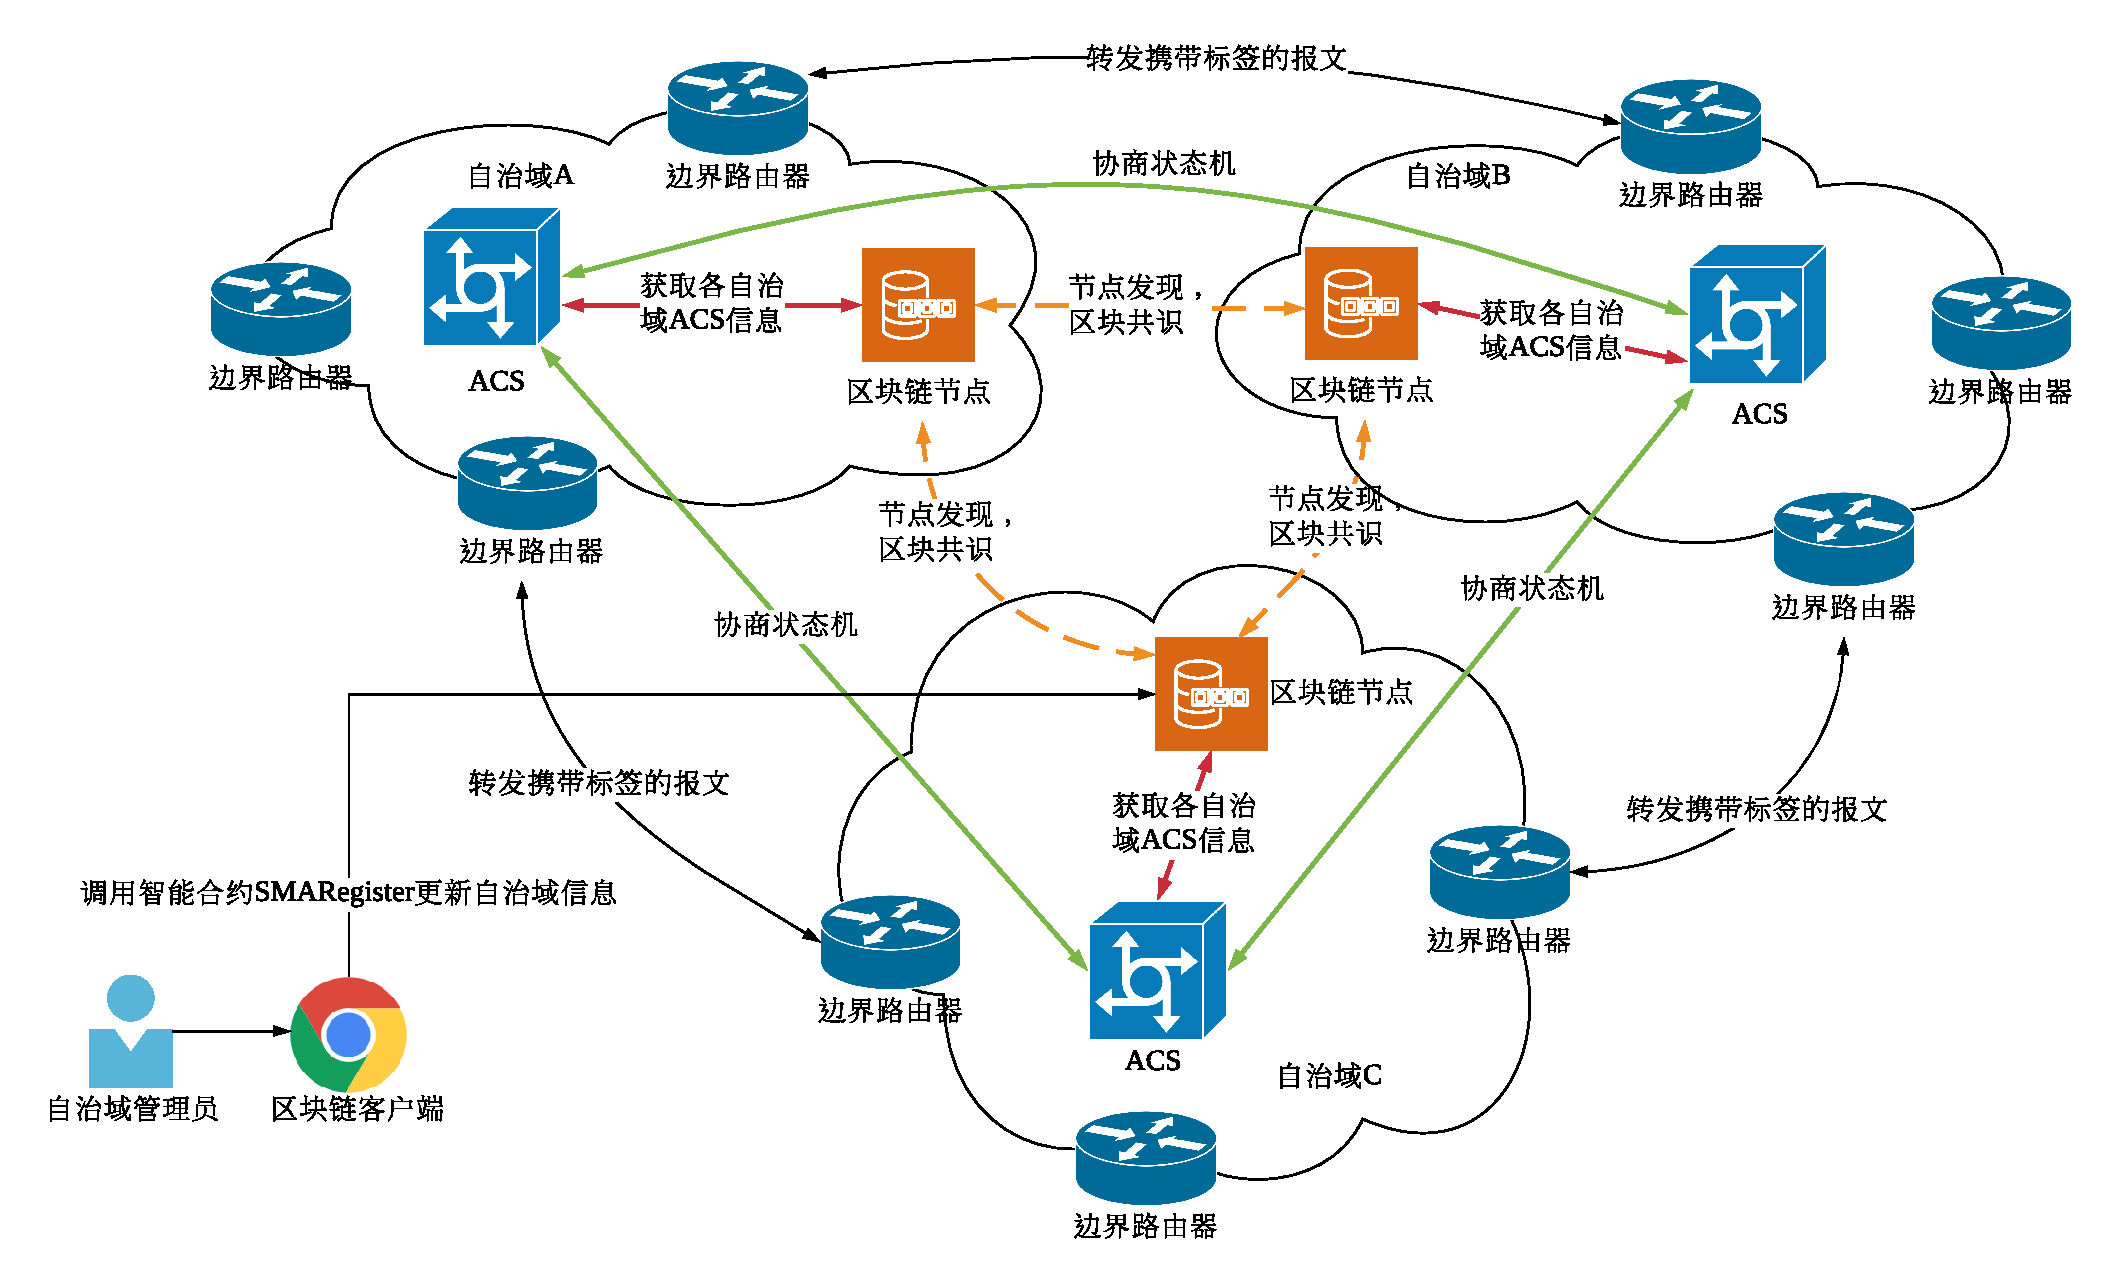
\includegraphics[width=\textwidth]{blockchain_sma_register_architecture.pdf}
        \caption{SMA联盟注册系统的区块链设计架构}
        \label{fig:blockchain_sma_register_architecture}
      \end{figure}

      在SMA原本的设计中,自治域信息更新采取部署SMA方案的自治域的管理员在线下向联盟管理员提交申请,联盟管理员审批后在REG服务器中进行手动维护的模式。本文将其变更为通过区块链提交申请,联盟管理员在链上对其申请进行审批的模式,从而规范化这一过程,并且保证自治域信息的更迭历史也可以得到保护和审计。
      此外,SMA采用REG定期向各ACS发送心跳以探测ACS状态并更新ACS信息列表,但采用区块链架构后由于区块链上的智能合约执行是一个多节点共识的过程,难以执行类似于单节点执行应用程序并通过API与外部系统进行交互的操作,因此本文设计了由ACS主动向联盟注册系统区块链定期拉取ACS信息列表的方式,将联盟注册信息的维护与更新两者解耦,由各自治域负责使用客户端向RegChain轮询最新的联盟ACS信息。

      本文设计了两个智能合约实现RegChain功能,分别命名为SMARegister与ASInfo。其中SMARegister由联盟管理员在启用联盟注册系统区块链第一个节点后进行部署,其所需要维护的内部状态如表\ref{tab:contract_SMARegister}所示。其中ASRequest为携带自治域信息的结构体,记录了自治域加入或离开安全联盟时提交申请的信息,包括申请类型、自治域号以及其他自治域相关信息等。ASInfo由SMARegister通过自治域申请时为自治域生成并部署,记录了特定自治域的信息以及ACS更新列表,其结构如表\ref{tab:contract_ASInfo}所示,其中AddrTime为一个包含ACS的IPv6地址与生效时间的二元组,类型为(String, Integer)。

      \begin{table}[htb]
        \centering
        \begin{minipage}[t]{\linewidth} 
          \caption{合约SMARegister信息列表}
          \label{tab:contract_SMARegister}
          \begin{tabularx}{\linewidth}{>{\centering\arraybackslash}X>{\centering\arraybackslash}X>{\centering\arraybackslash}X}
            \toprule[1.5pt]
            {\heiti 属性名} & {\heiti 类型} & {\heiti 说明} \\\midrule[1pt]
            req\_queue & ASRequest Array & 待审批的自治域信息更新请求列表 \\ 
            as\_queue & ASInfo Array & 自治域合约列表 \\
            \bottomrule[1.5pt]
          \end{tabularx}
        \end{minipage}
      \end{table}
      
      \begin{table}[htb]
        \centering
        \begin{minipage}[t]{\linewidth} 
          \caption{合约ASInfo信息列表}
          \label{tab:contract_ASInfo}
          \begin{tabularx}{\linewidth}{>{\centering\arraybackslash}X>{\centering\arraybackslash}X>{\centering\arraybackslash}X}
            \toprule[1.5pt]
            {\heiti 属性名} & {\heiti 类型} & {\heiti 说明} \\\midrule[1pt]
            id & String & 唯一标识自治域的标识符 \\ 
            asn & Integer & 自治域号 \\
            name & String & 自治域名 \\
            description & String & 自治域详细信息 \\
            acs\_queue & AddrTime Array & 自治域ACS信息列表 \\
            \bottomrule[1.5pt]
          \end{tabularx}
        \end{minipage}
      \end{table}

      本文在尽可能与原协议设计保持一致的情况下,设计各功能基于区块链的实现如下,均由SMARegister与ASInfo合约提供函数给各自治域管理员与ACS进行调用:
      \begin{enumerate}[1{)}]
        \item \textbf{自治域申请}:在自治域加入或离开SMA安全联盟时,填写自治域相关信息,包括申请类型、自治域号、自治域名称、详细信息,签发交易调用SMARegister的自治域申请函数,由SMARegister将其加入req\_queue中,等待联盟管理员审核。联盟管理员可通过SMARegister提供的查询函数查看已有的申请,当需要批准或拒绝申请时,其使用联盟管理的私钥签发交易调用SMARegister的函数进行批准或拒绝。审批通过的自治域将生成一个新的ASInfo合约加入as\_queue中并部署在区块链上,为该自治域提供ACS更新服务。
        \item \textbf{自治域ACS更新}:自治域管理员填写ACS的IPv6地址、配置生效时间等信息,使用自治域私钥签发交易广播给RegChain网络,交易中包含对其管理的ASInfo合约提供的自治域ACS更新函数的调用。ACS更新的操作将自动执行,不需要等待联盟管理员的审批,从而增加SMA控制平面信息更新的便捷性。
        \item \textbf{ACS信息同步}:ACS信息的定期同步功能由REG移交到各自治域的ACS,ACS周期性调用SMARegister提供的查询接口,更新本地的联盟ACS信息列表。由于仅对数据进行查询,不需要向区块链中写入新数据,因此ACS信息同步可以即时完成,不需要等待区块链的下一次出块。
      \end{enumerate}

      \subsubsection{自治域申请审批机制}
      \label{IPv6_Security:interas:design:update}
      自治域申请发生在有新的自治域部署SMA方案或已部署的自治域离开SMA安全联盟时,本文设计自治域申请的格式如表\ref{tab:blockchain_design_as_request}所示,将其称为ASRequest。
      \begin{table}[htb]
        \centering
        \begin{minipage}[t]{\linewidth} 
          \caption{自治域申请ASRequest格式}
          \label{tab:blockchain_design_as_request}
          \begin{tabularx}{\linewidth}{cc>{\centering\arraybackslash}X>{\centering\arraybackslash}X}
            \toprule[1.5pt]
            {\heiti 名称} & {\heiti 类型} & {\heiti 举例} & {\heiti 说明} \\\midrule[1pt]
            req\_type & Enum & Register & 指示自治域申请类型的枚举,包含Register与Delete  \\ 
            asn & Integer & 45576 & 自治域号 \\
            name & String & CERNET2-TSINGHUA6-AS-AP & 自治域名称 \\
            description & String & Tsinghua University & 自治域的详细信息 \\
            \bottomrule[1.5pt]
          \end{tabularx}
        \end{minipage}
      \end{table}

      其中,req\_type用于指示本次申请的类型,分为Register与Delete两种。为了便于自治域信息的查找与更新权限控制,在自治域注册申请被联盟管理员批准后,SMARegister将为其部署一个新的ASInfo合约,以该次交易的钱包地址作为所有者,与该自治域的AS号进行绑定,后续对合约进行更新的交易必须由同一地址的账户发起。

      自治域管理员填写自治域申请后,经由客户端签发交易并广播,调用智能合约SMARegister提供的自治域申请函数,本文将其命名为createASRequest。RegChain中的节点收到该交易后进行共识,调用各自维护的SMARegister执行相关调用。createASRequest将自治域申请加入到req\_queue中等待联盟管理员审批,并不直接更新as\_queue队列。联盟管理员通过调用SMARegister的requestQuery接口查看待审批列表,对自治域申请进行审批,分别调用SMARegister的requestApprove与requestReject函数进行批准或拒绝。经过批准的自治域信息将被用于生成一个新的ASInfo合约,并加入到as\_queue中。自治域申请与审批的时序如图\ref{fig:blockchain_as_update_procedure}所示。
      
      \begin{figure}[ht]
        \centering
        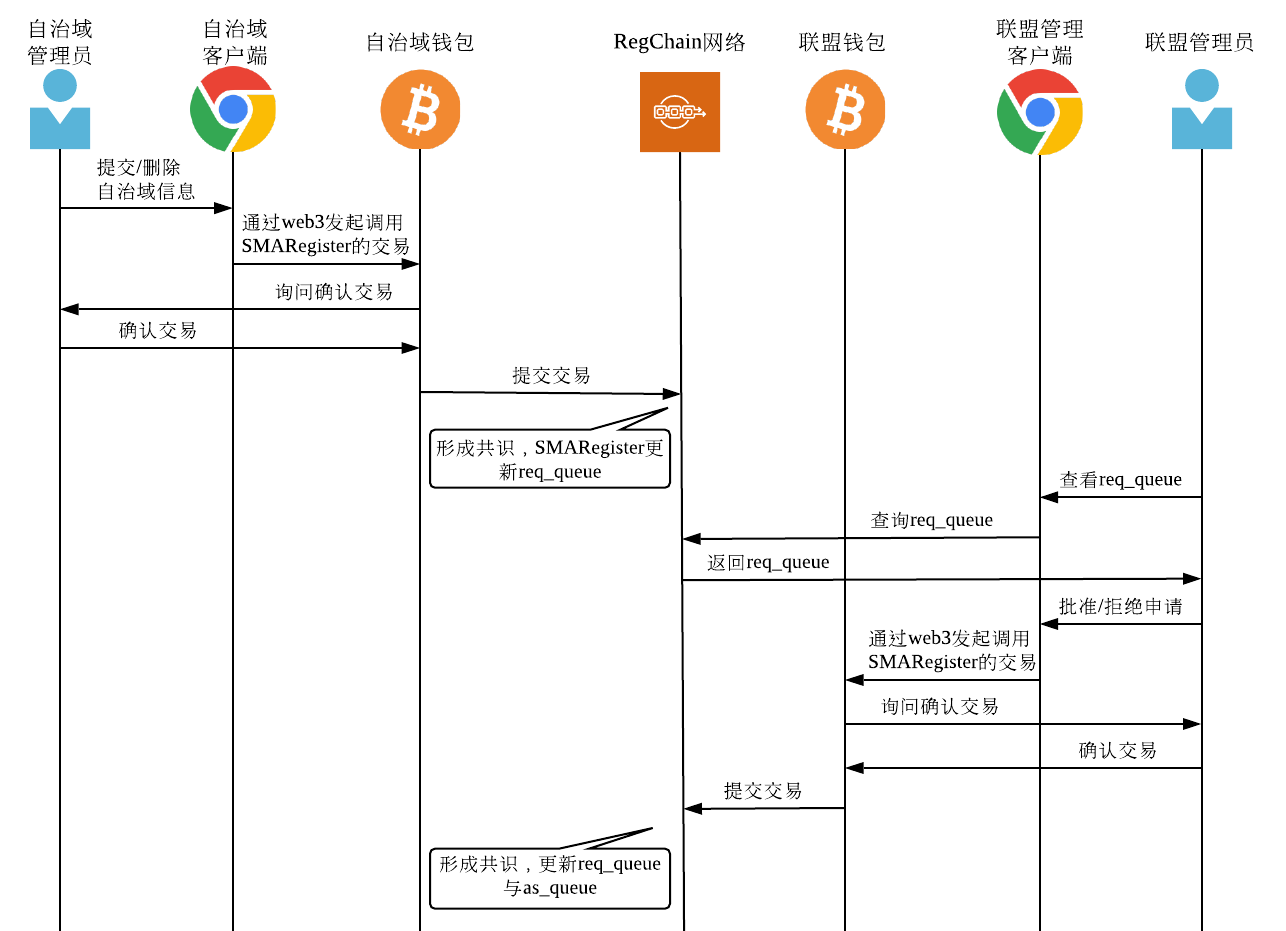
\includegraphics[width=\textwidth]{blockchain_as_update_procedure.png}
        \caption{RegChain自治域申请时序}
        \label{fig:blockchain_as_update_procedure}
      \end{figure}

      SMARegister为自治域申请审批机制提供的相关函数总结如表\ref{tab:contract_as_request_function}所示。

      \begin{table}[htb]
        \centering
        \begin{minipage}[t]{\linewidth} 
          \caption{SMARegister自治域申请审批相关函数}
          \label{tab:contract_as_request_function}
          \begin{tabularx}{\linewidth}{cccc>{\centering\arraybackslash}X}
            \toprule[1.5pt]
            {\heiti 函数名} & {\heiti 参数类型} & {\heiti 返回类型} & {\heiti 调用者} & {\heiti 说明} \\\midrule[1pt]
            createASRequest & ASRequest & 无 & 自治域管理员 & 提交自治域申请 \\ 
            requestQuery & 无 & ASRequest Array & 联盟管理员 & 查看待审批的自治域申请列表 \\ 
            requestApprove & String & 无 & 联盟管理员 & 接收自治域标识,通过其对应AS的申请 \\ 
            requestReject & String & 无 & 联盟管理员 & 接收自治域标识,拒绝其对应AS的申请 \\ 
            \bottomrule[1.5pt]
          \end{tabularx}
        \end{minipage}
      \end{table}

      \subsubsection{自治域ACS更新机制}
      在自治域申请经过联盟管理员批准后,该自治域将拥有一个独立的ASInfo合约记录其信息并提供ACS更新服务。自治域管理员可通过其申请时的钱包地址自主调用updateACS函数进行ACS配置的更新,而无需调用SMARegister要求联盟管理员的批准。

      由于自治域ACS信息并不即时生效,可能在将来某个时间点才发生切换,因此ASInfo必须将ACS的历次更新均记录下来,以供后续配置的平滑切换,而不是简单地记录一个ACS的最新信息,因此表\ref{tab:contract_ASInfo}中使用了acs\_queue对其进行记录。当有新的ACS配置更新时,先前生效时间晚于其生效时间的ACS配置将自动失效,其更新算法如算法\ref{algo:blockchain_as_update}所示。

      \begin{algorithm}
        \caption{RegChain自治域ACS更新算法}
        \label{algo:blockchain_as_update}
        
        \LinesNumbered
        \SetKw{KwInList}{in}
        \SetKw{KwDownto}{downto}

        \SetKw{KwBreak}{break}
        \SetKw{KwReturn}{return}
        
        \SetKw{KwTrue}{true}
        \SetKw{KwFalse}{false}
        
        \SetKw{KwAnd}{and}
        \SetKw{KwNot}{not}
        
        \SetKw{KwAssert}{assert}
        \SetKw{KwNew}{new}


        \KwIn{acs\_addr, effect\_time}

        new\_pair \gets \KwNew AddrTime(acs\_addr, effect\_time)\;
        \While{as\_info.acs\_queue.length() > 0} {
            last\_time \gets as\_info.acs\_queue.lastElement().effect\_time\;
            \If{effect\_time <= last\_time} {
                as\_info.acs\_queue.removeLastElement()\;
            }
            \Else {
                \KwBreak\;
            }
        }
        as\_info.acs\_queue.add(new\_pair)\;
      \end{algorithm}


      \subsubsection{ACS信息同步机制}
      \label{IPv6_Security:interas:design:heartbeat}
      ACS信息同步机制由原先的REG主动推送修改为ACS主动查询。由于ACS向RegChain查询联盟ACS信息列表不需要向区块链中写入数据,因此其是一个即时操作,不需要各节点达成共识。本文设计SMARegister提供联盟内所有自治域的ASInfo列表查询函数ASQuery,并设计ASInfo合约提供查询该自治域当前有效ACS地址的函数getCurrentACS,两者如表\ref{tab:contract_as_query_function}所示。客户端进行ACS信息拉取时,首先向SMARegister获取所有自治域的ASInfo合约,然后分别对每个自治域进行当前ACS地址的获取。
      \begin{table}[htb]
        \centering
        \begin{minipage}[t]{\linewidth} 
          \caption{自治域信息查询相关函数}
          \label{tab:contract_as_query_function}
          \begin{tabularx}{\linewidth}{cccc>{\centering\arraybackslash}X}
            \toprule[1.5pt]
            {\heiti 合约名} & {\heiti 函数名} & {\heiti 参数类型} & {\heiti 返回类型} & {\heiti 说明} \\\midrule[1pt]
            SMARegister & ASQuery & 无 & ASInfo Array & 获取联盟内所有自治域的ASInfo合约 \\ 
            ASInfo & getCurrentACS & Integer & String & 提交当前查询时间,获取当前有效的ACS地址 \\ 
            \bottomrule[1.5pt]
          \end{tabularx}
        \end{minipage}
      \end{table}

      之所以要在getCurrentACS的参数中携带查询时的时间信息,是由于在EVM内部无法获知当前的确切时间,因此需要ACS主动将当前时间告知ASInfo,这一步骤由RegChain的客户端自动填充,不需要手动填写。ASInfo将根据查询时间,对维护的ACS信息列表进行从头到尾的扫描,以确定在该时间点生效的ACS信息,由于这一算法较为简单,故不再赘述。

    \subsection{基于以太坊的SMA联盟注册系统实现}
    \label{IPv6_Security:interas:implement}
    SMA联盟注册系统的主要功能是自治域信息的更新与查询,由于现实网络中为了维持域间报文转发的稳定,自治域管理员并不会频繁更新自治域ACS的地址,且其更新操作中携带有配置的生效时间,一般发生在未来若干小时甚至若干天后,因此对于更新的实时性没有特别高的要求。查询操作要求很高的实时性,但由于其不需要向区块链中写入数据,因此可以实时返回结果,与区块链采用的共识算法无关。另一方面,倘若采用Raft等共识算法,虽然可以提高共识效率,但却以牺牲对恶意节点接入的防御能力为代价,从而使SMA联盟注册系统的安全性大打折扣。综上考虑,本文选择PoW作为共识算法,采用以太坊平台实现RegChain,项目代码参见RegChain的Git仓库\footnote{RegChain repository, https://github.com/BragCat/RegChain}。

      \subsubsection{整体架构}
      \label{IPv6_Security:interas:implement:architecture}
      为了实现对用户的友好,本文的客户端采用React\footnote{React, https://zh-hans.reactjs.org/docs/getting-started.html}开发,自治域管理员只需要使用浏览器并安装一个钱包插件即可使用,而无需安装特殊的客户端。希望能够参与网络共识的自治域,可以在本地部署一个以太坊节点,以更稳定地提供共识与接入服务,以太坊节点可选择Parity\footnote{Parity, https://www.parity.io/ethereum/}、Geth\footnote{Geth, https://geth.ethereum.org/}等任意一款支持运行完整以太坊节点的软件。客户端通过Web3.js\footnote{Web3, https://github.com/ethereum/wiki/wiki/JavaScript-API}连接到区块链节点进行数据的读写,其架构方式与传统网络应用的对比如图\ref{fig:blockchain_tradition_ethereum_comparison}所示,在以太坊构建的应用中,Web3.js相当于传统应用中的后端,本文将使用Web3.js的API开发相应的逻辑进行连接区块链节点、构建交易、读写区块链数据等交互操作。区块链网络相当于传统应用中对应的数据库,但其提供了更高的可用性与更加强大的安全特性。

      \begin{figure}[ht]
        \centering
        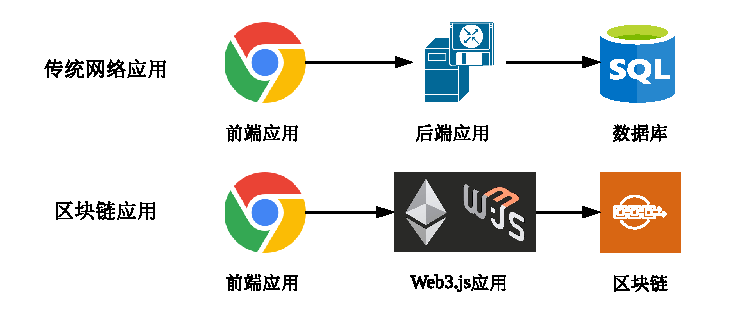
\includegraphics[width=0.8\textwidth]{blockchain_tradition_ethereum_comparison.pdf}
        \caption{传统网络应用与以太坊应用架构对比}
        \label{fig:blockchain_tradition_ethereum_comparison}
      \end{figure}

      RegChain的以太坊实现包含图\ref{fig:blockchain_regchain_implementation}所示的两个部分,一部分为使用React框架开发的网页客户端,主要包括联盟管理员查看与审批申请、自治域管理员提交请求等功能,自治域管理员与联盟管理员只需要在Chrome浏览器或Firefox浏览器上安装支持以太坊的钱包插件,如MetaMask,即可使用浏览器访问React App提供的页面并进行操作;另一部分为将自治域信息查询功能封装后的Javascript包,提供联盟内ACS信息的拉取服务,其内部调用Web3.js与区块链进行交互,向外提供查询自治域ACS信息的接口,自治域ACS调用其接口即可向区块链查询获得联盟内所有自治域当前有效的ACS地址。两个部分共享同一个后端服务,即RegChain区块链上的智能合约SMARegister与各个自治域对应的ASInfo。
      
      \begin{figure}[ht]
        \centering
        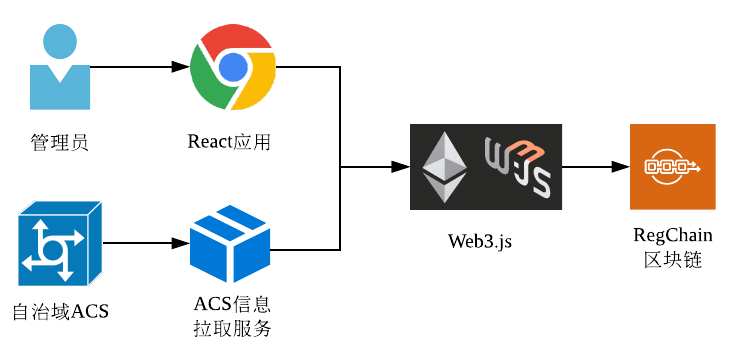
\includegraphics[width=0.8\textwidth]{figures/blockchain_regchain_implementation.png}
        \caption{SMA联盟注册系统的以太坊实现架构}
        \label{fig:blockchain_regchain_implementation}
      \end{figure}

      \subsubsection{DApp}
      \label{IPv6_Security:interas:implement:dapp}
      DApp是具有执行能力的应用代码,其以智能合约的形式部署在每一个以太坊节点上,每个节点对于新区块中的交易,依次执行智能合约的调用,各自独立维护合约内部状态。由于所有执行步骤的确定性,最终每个以太坊节点上合约状态都将保持一致,相当于同一个应用分布在整个网络的节点上执行,保持了应用的多个副本,因此被称为分布式应用。本文采用Truffle\footnote{Truffle, https://www.trufflesuite.com/docs}工具链开发与测试DApp。
      
      SMA联盟注册系统的DApp主要需要实现智能合约SMARegister与ASInfo,两者需要维护的内部状态已由表\ref{tab:contract_SMARegister}与表\ref{tab:contract_ASInfo}定义,本文在使用Solidity进行实现时,由于Solidity语言的一些限制,因此与原设计有所区别。
      SMARegister中两个数组即对应了Solidity中的动态数组类型,但对ASRequest结构体做了一些更改,如表\ref{tab:ethereum_ASRequest_attributes}所示。ASInfo中各属性除ACS列表外均由ASRequest生成,在此不再赘述。
      \begin{table}[htb]
        \centering
        \begin{minipage}[t]{\linewidth} 
          \caption{ASRequest数据结构}
          \label{tab:ethereum_ASRequest_attributes}
          \begin{tabularx}{\linewidth}{cc>{\centering\arraybackslash}X>{\centering\arraybackslash}X}
            \toprule[1.5pt]
            {\heiti 属性名} & {\heiti 原类型} & {\heiti Solidity数据结构} & {\heiti 说明} \\\midrule[1pt]
            owner & 未定义 & address & 发起申请交易的钱包地址 \\
            id & String & bytes20 & 根据owner生成的自治域标识 \\
            req\_type & Enum & uint256 & 0表示Register,1表示Delete \\ 
            asn & Integer & uint256 & 自治域号 \\
            name & String & string & 自治域名 \\
            description & String & string & 自治域详细信息 \\
            \bottomrule[1.5pt]
          \end{tabularx}
        \end{minipage}
      \end{table}

      之所以需要将自治域标识id与ASInfo的所有者owner进行分别存储,是由于Javascript没有Solidity的address所对应的类型,在客户端通过自治域标识进行对应自治域申请审批时无法直接发送address类型的数据,因此只能使用字符串存储id以与客户端兼容。同时,由于Solidity暂时不支持返回结构体数组,比如string[],因此必须将id定义为bytes20而非变长的string类型以支持requestQuery函数查询当前所有的自治域申请。

      SMARegister与ASInfo实现了\ref{IPv6_Security:interas:design}节中提到的各函数,并采用了modifier对函数调用者身份进行限定,仅允许SMARegister的部署者即联盟管理员调用requestApprove与requestReject函数,仅允许ASInfo的所有者调用updateACS函数。
    
      图\ref{fig:regchain_dapp_tx}展示了RegChain在实验中的一些交易历史,从头至尾查看历次交易即可获知RegChain所经历的所有历史状态。为了审计的便利性,本文在实现DApp时还利用以太坊的事件机制,设计了ASCreated、ASRequestApproved等多个事件,如图\ref{fig:regchain_dapp_event}所示,在RegChain网络执行合约时将根据交易的调用生成相应的事件形成日志,便于查看RegChain中各自治域的变更历史。

      \begin{figure}[H]
        \centering
        \subcaptionbox{RegChain交易历史\label{fig:regchain_dapp_tx}}
        {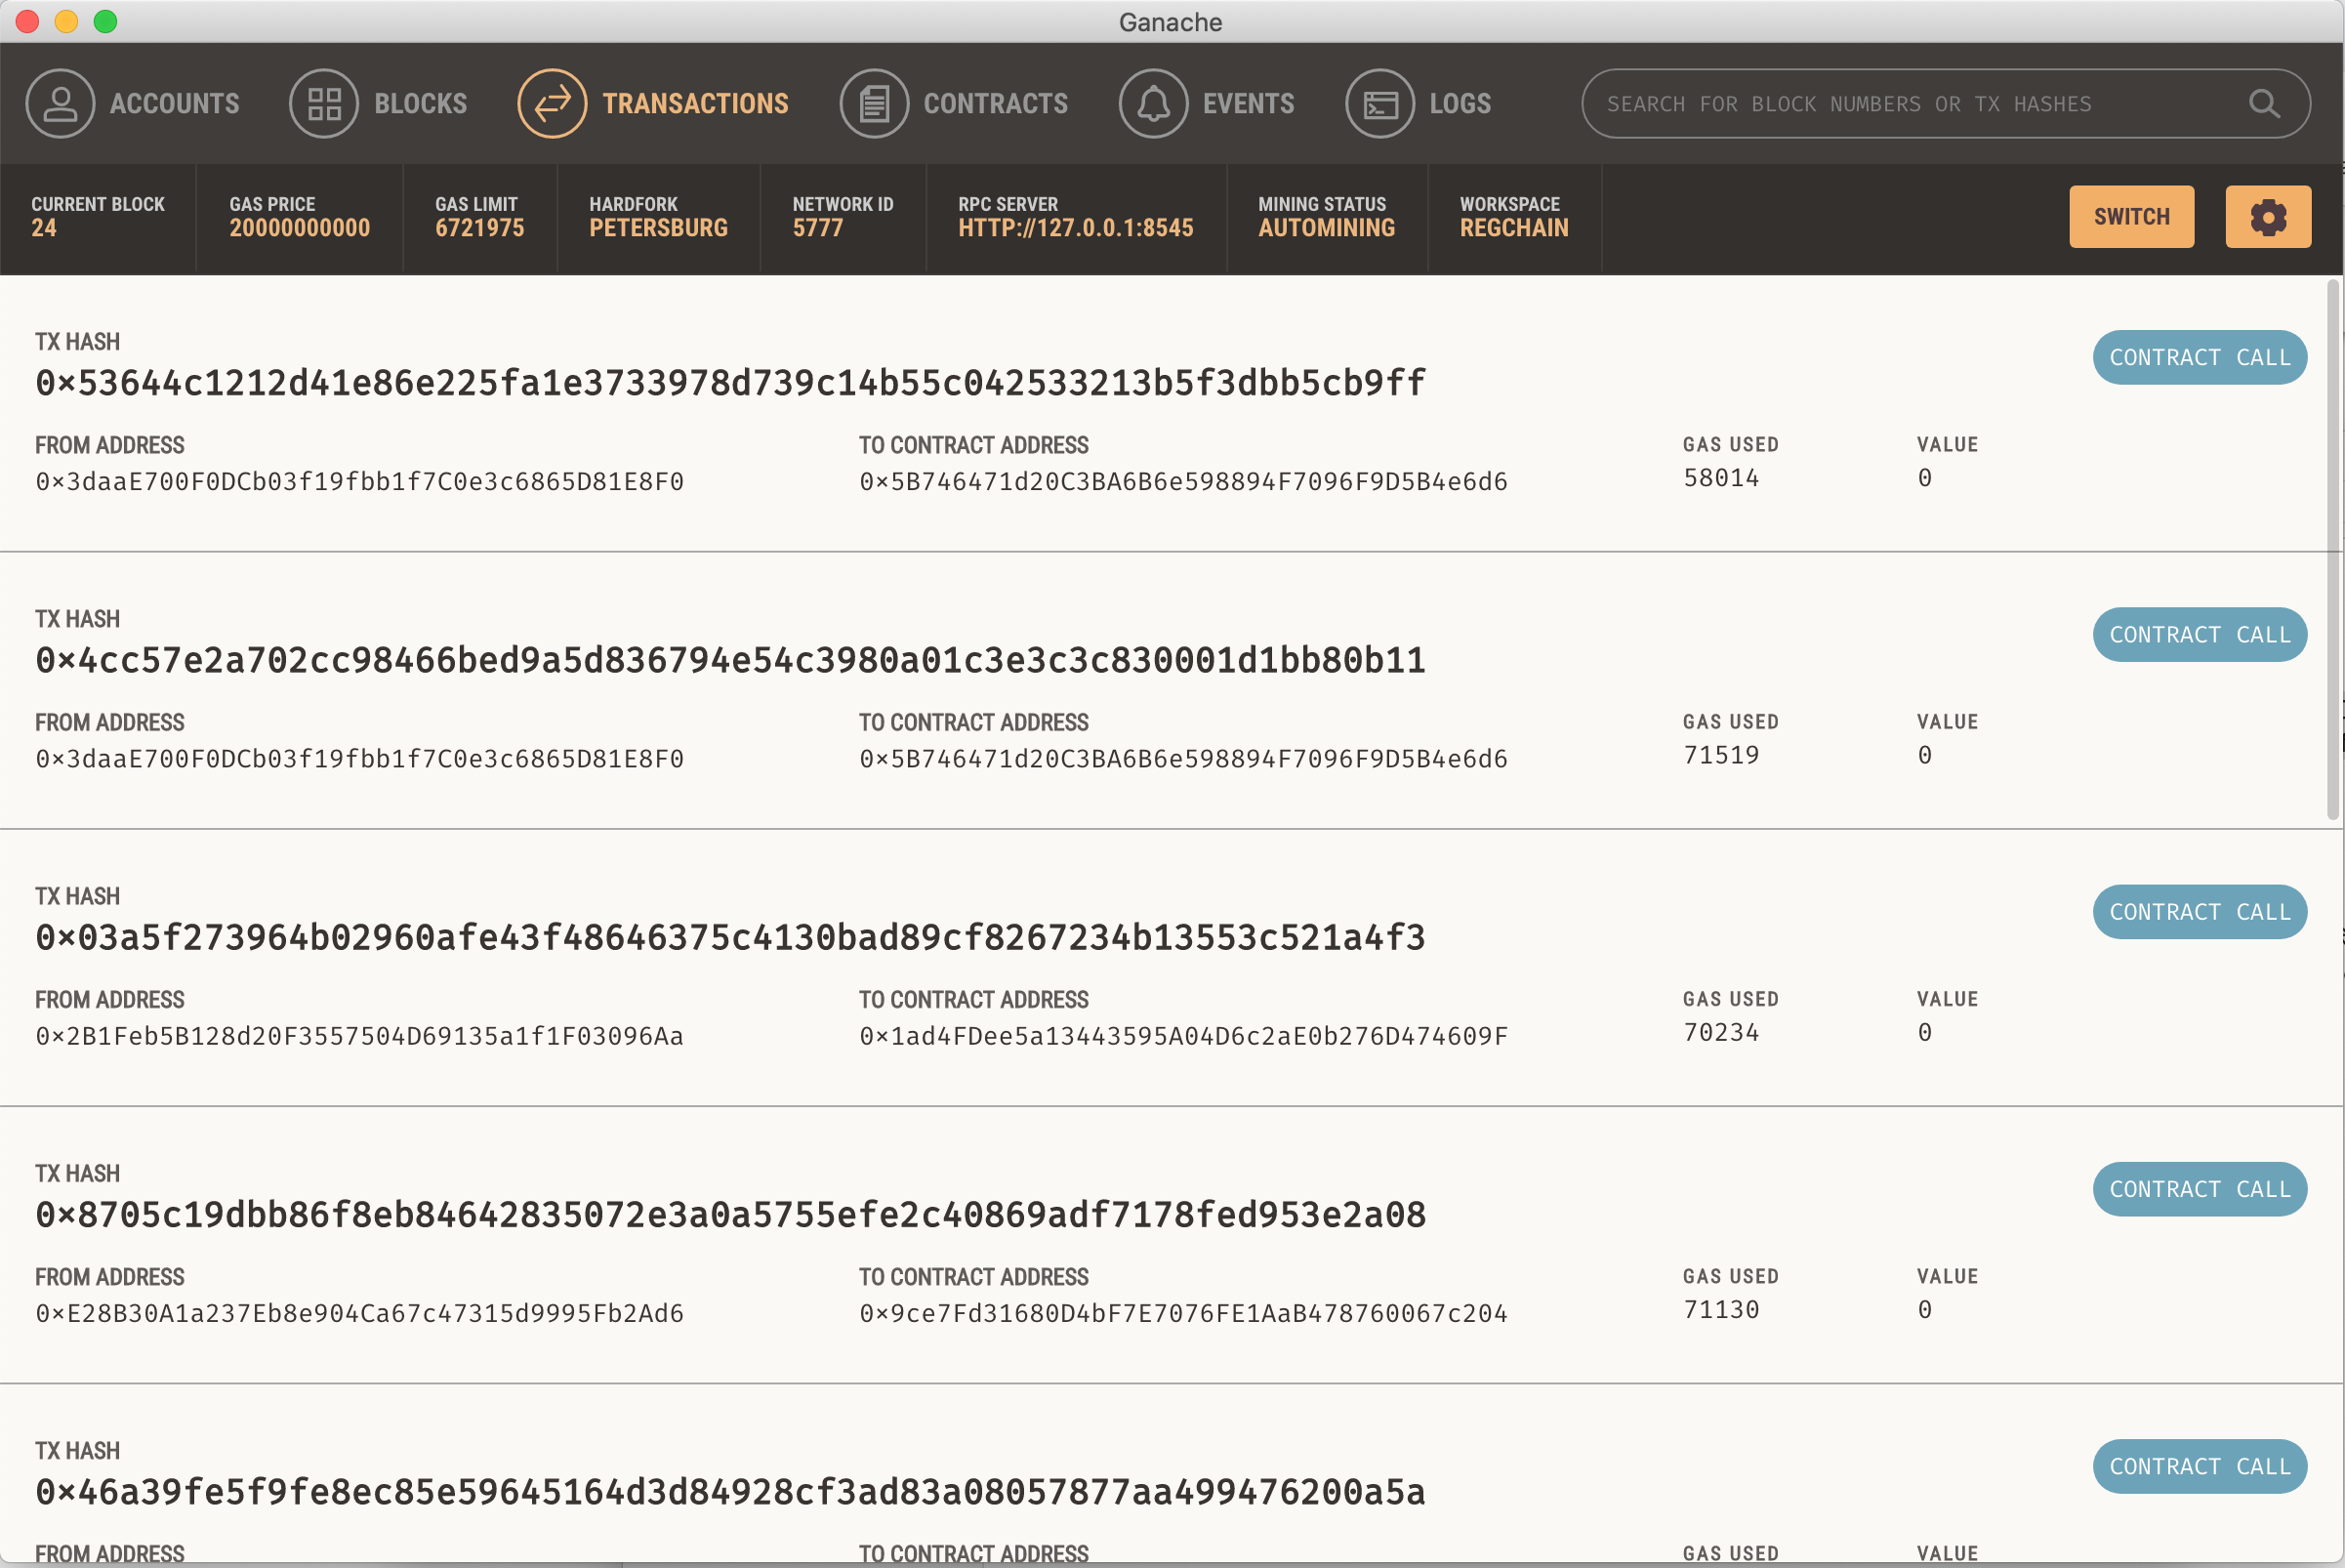
\includegraphics[height=4.8cm]{figures/regchain_dapp_tx.png}}
        \hspace{1em}
        \subcaptionbox{RegChain事件历史\label{fig:regchain_dapp_event}}
        {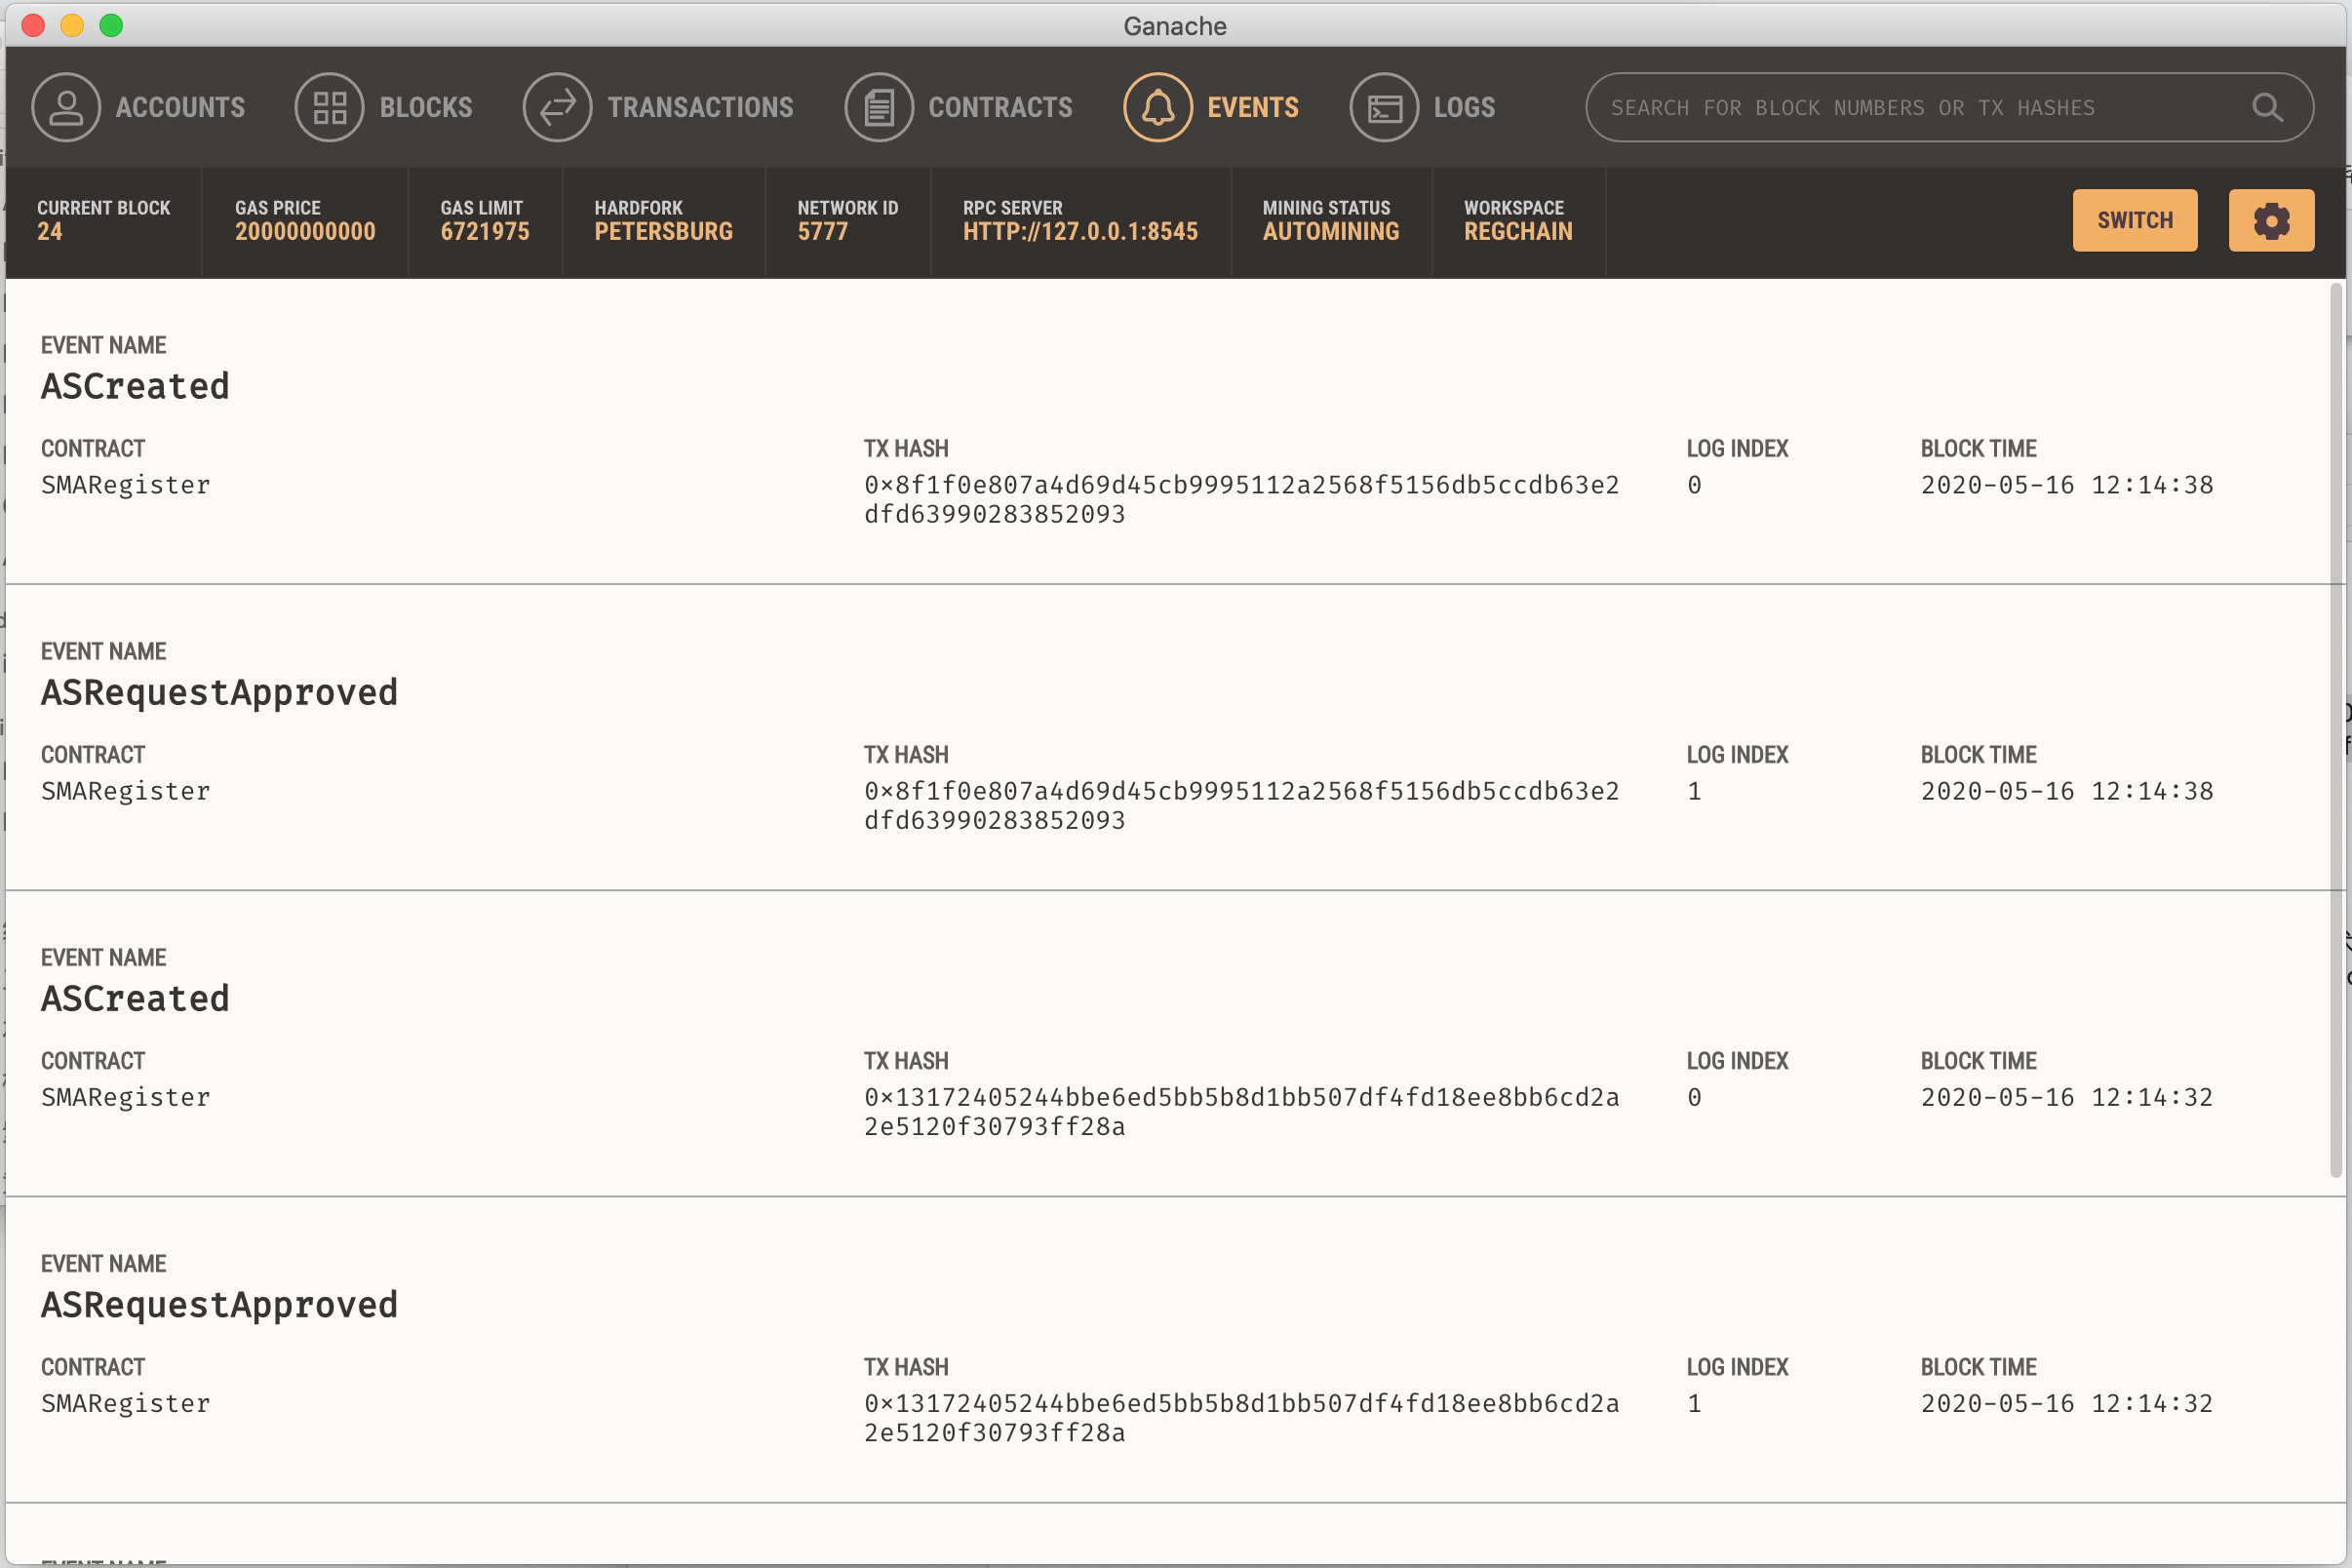
\includegraphics[height=4.8cm]{figures/regchain_dapp_event.png}}
        \caption{RegChain DApp端交易与事件展示}
        \label{fig:regchain_dapp_images}
      \end{figure}


      \subsubsection{客户端}
      \label{IPv6_Security:interas:implement:client}
      本文在客户端处的实现包含网页客户端与ACS信息拉取服务。
      
      网页客户端由React框架实现,提供自治域管理员与联盟管理员查看与操作RegChain的浏览器页面,两者的回调函数分别如表\ref{tab:sma_admin_client_callback_function}与表\ref{tab:sma_as_client_callback_function}所示。
      \begin{table}[htb]
        \centering
        \begin{minipage}[t]{\linewidth} 
          \caption{SMA联盟注册系统以太坊实现的联盟管理客户端回调函数}
          \label{tab:sma_admin_client_callback_function}
          \begin{tabularx}{\linewidth}{cc>{\centering\arraybackslash}X}
            \toprule[1.5pt]
            {\heiti 函数名} & {\heiti 参数名} & {\heiti 说明} \\\midrule[1pt]
            handleSubmitApprove & id & 联盟管理员点击自治域申请通过按钮的回调函数,调用SMARegister.requestApprove函数通过申请 \\ 
            handleSubmitReject & id & 联盟管理员点击自治域申请拒绝按钮的回调函数,调用SMARegister.requestReject函数拒绝申请 \\
            \bottomrule[1.5pt]
          \end{tabularx}
        \end{minipage}
      \end{table}
      
      \begin{table}[htb]
        \centering
        \begin{minipage}[t]{\linewidth} 
          \caption{SMA联盟注册系统以太坊实现的自治域客户端回调函数}
          \label{tab:sma_as_client_callback_function}
          \begin{tabularx}{\linewidth}{c>{\centering\arraybackslash}X>{\centering\arraybackslash}X}
            \toprule[1.5pt]
            {\heiti 函数名} & {\heiti 参数名} & {\heiti 说明} \\\midrule[1pt]
            handleSubmitRequest & req\_type, asn, name, description & 自治域管理员点击自治域申请提交按钮的回调函数,调用SMARegister.createASRequest提交申请 \\ 
            handleSubmitUpdate & acs\_addr, effect\_time & 自治域管理员点击自治域ACS更新提交按钮的回调函数,调用ASInfo.updateACS更新ACS配置 \\ 
            \bottomrule[1.5pt]
          \end{tabularx}
        \end{minipage}
      \end{table}


      
      自治域管理员进行自治域申请的页面如图\ref{fig:regchain_client_request}所示,可通过点击“自治域变更”进行自治域信息的填写。当自治域管理员点击提交按钮时,MetaMask将弹出询问是否允许使用当前账户进行交易签名。
      
      \begin{figure}[H]
        \centering
        \subcaptionbox{申请填写与提交\label{fig:regchain_client_request_1}}
        {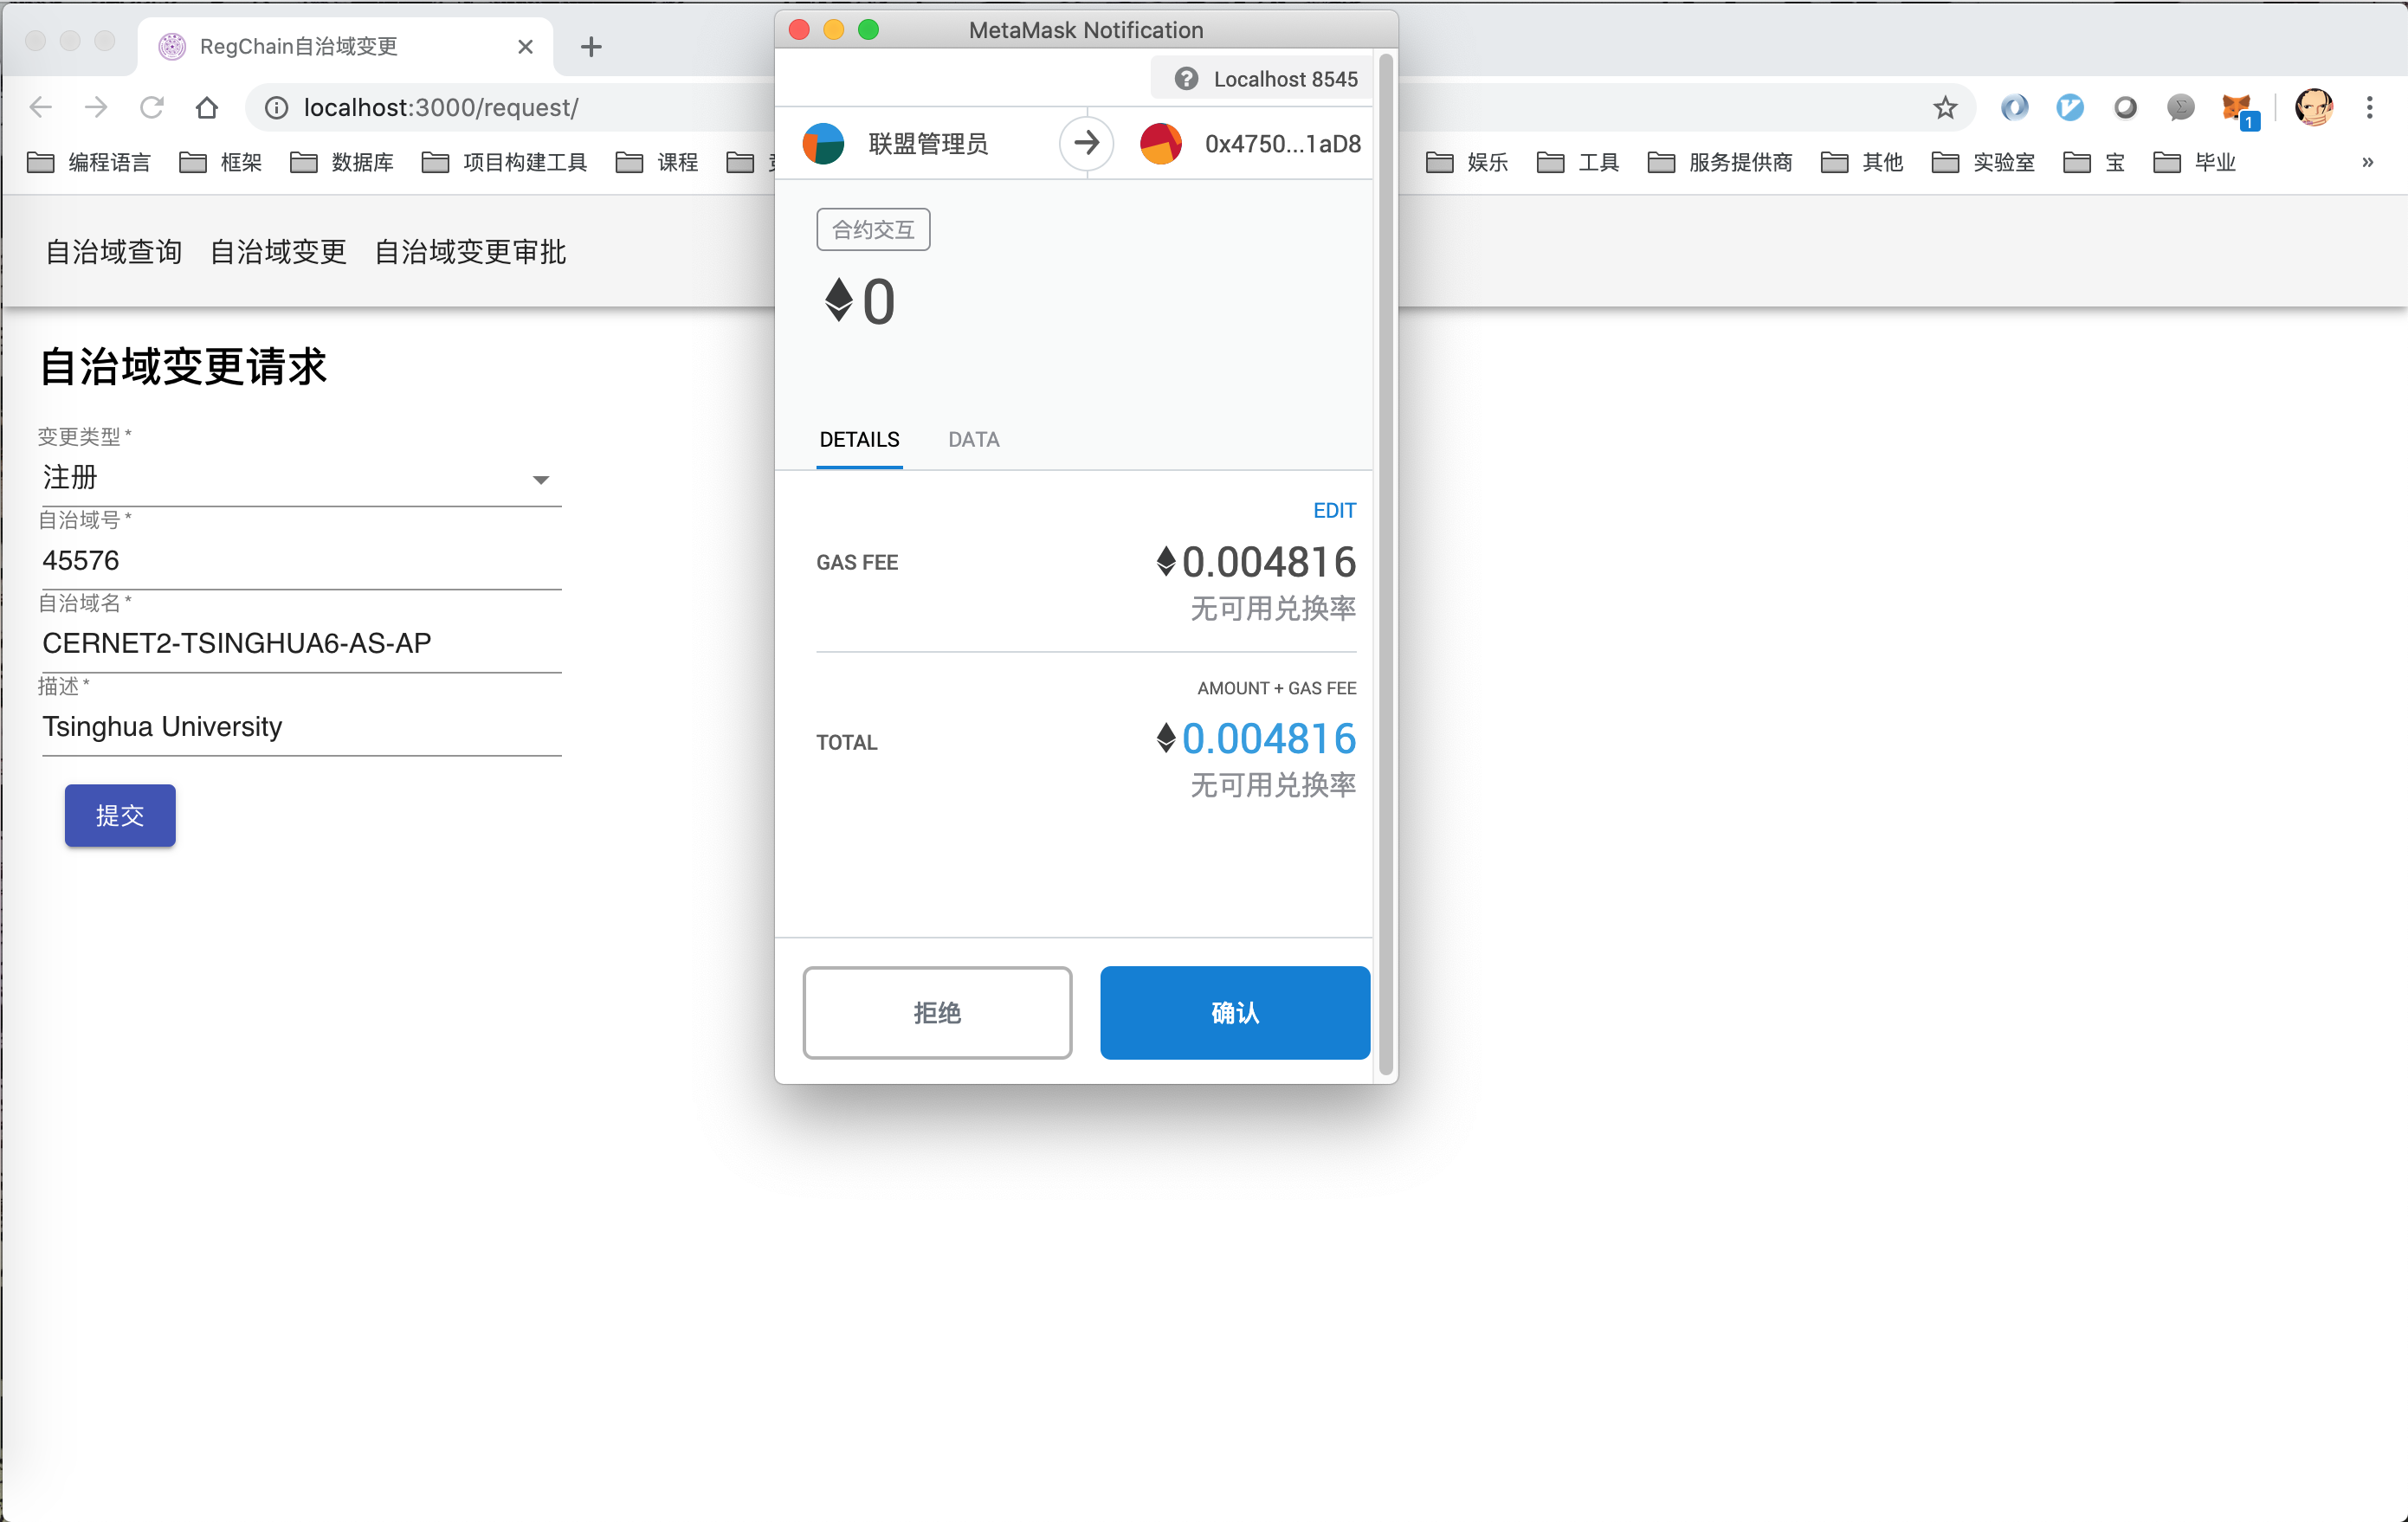
\includegraphics[height=4.5cm]{figures/regchain_client_request_1.png}}
        \hspace{1em}
        \subcaptionbox{申请提交成功\label{fig:regchain_client_request_2}}
        {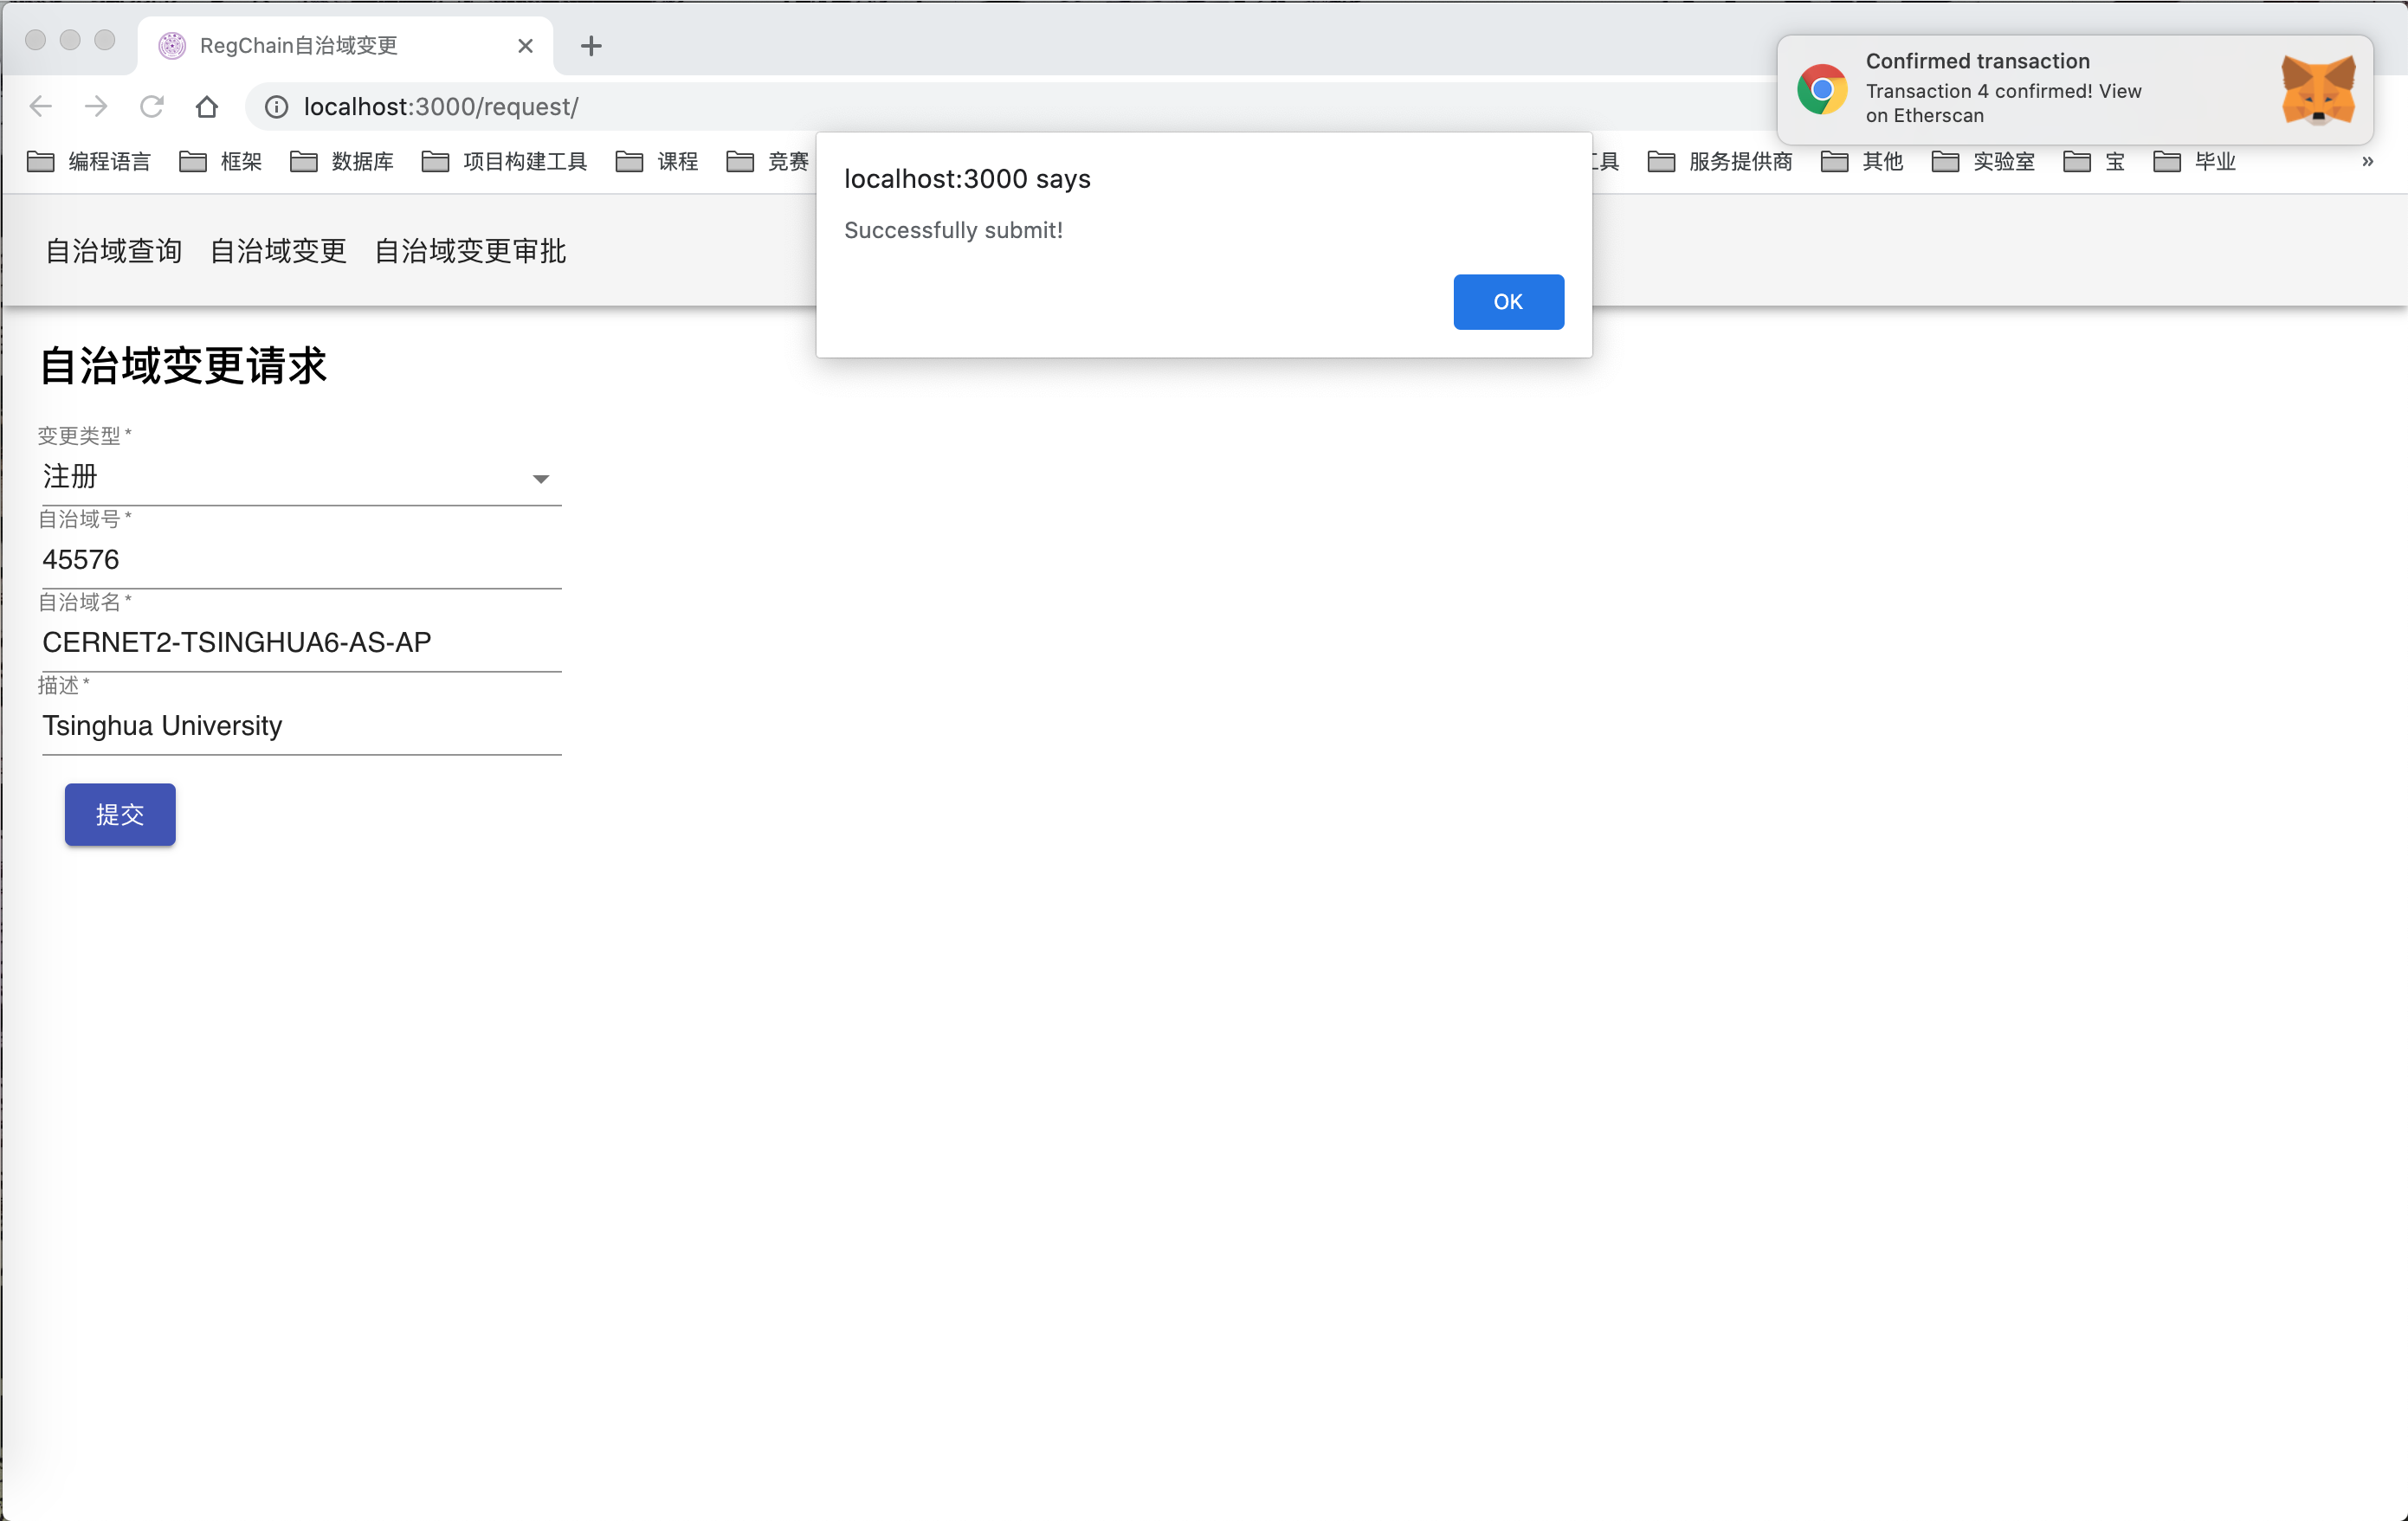
\includegraphics[height=4.5cm]{figures/regchain_client_request_2.png}}
        \caption{RegChain自治域申请页面}
        \label{fig:regchain_client_request}
      \end{figure}
      
      联盟管理员可通过“自治域变更审批”查看当前提交的自治域申请,并使用通过或拒绝按钮审批相应的申请,如图\ref{fig:regchain_client_review_1}所示。当非联盟管理员使用其他钱包尝试进行审批时,将被SMARegister所阻止,如图\ref{fig:regchain_client_review_2}所示。

      \begin{figure}[H]
        \centering
        \subcaptionbox{管理员正常审批\label{fig:regchain_client_review_1}}
        {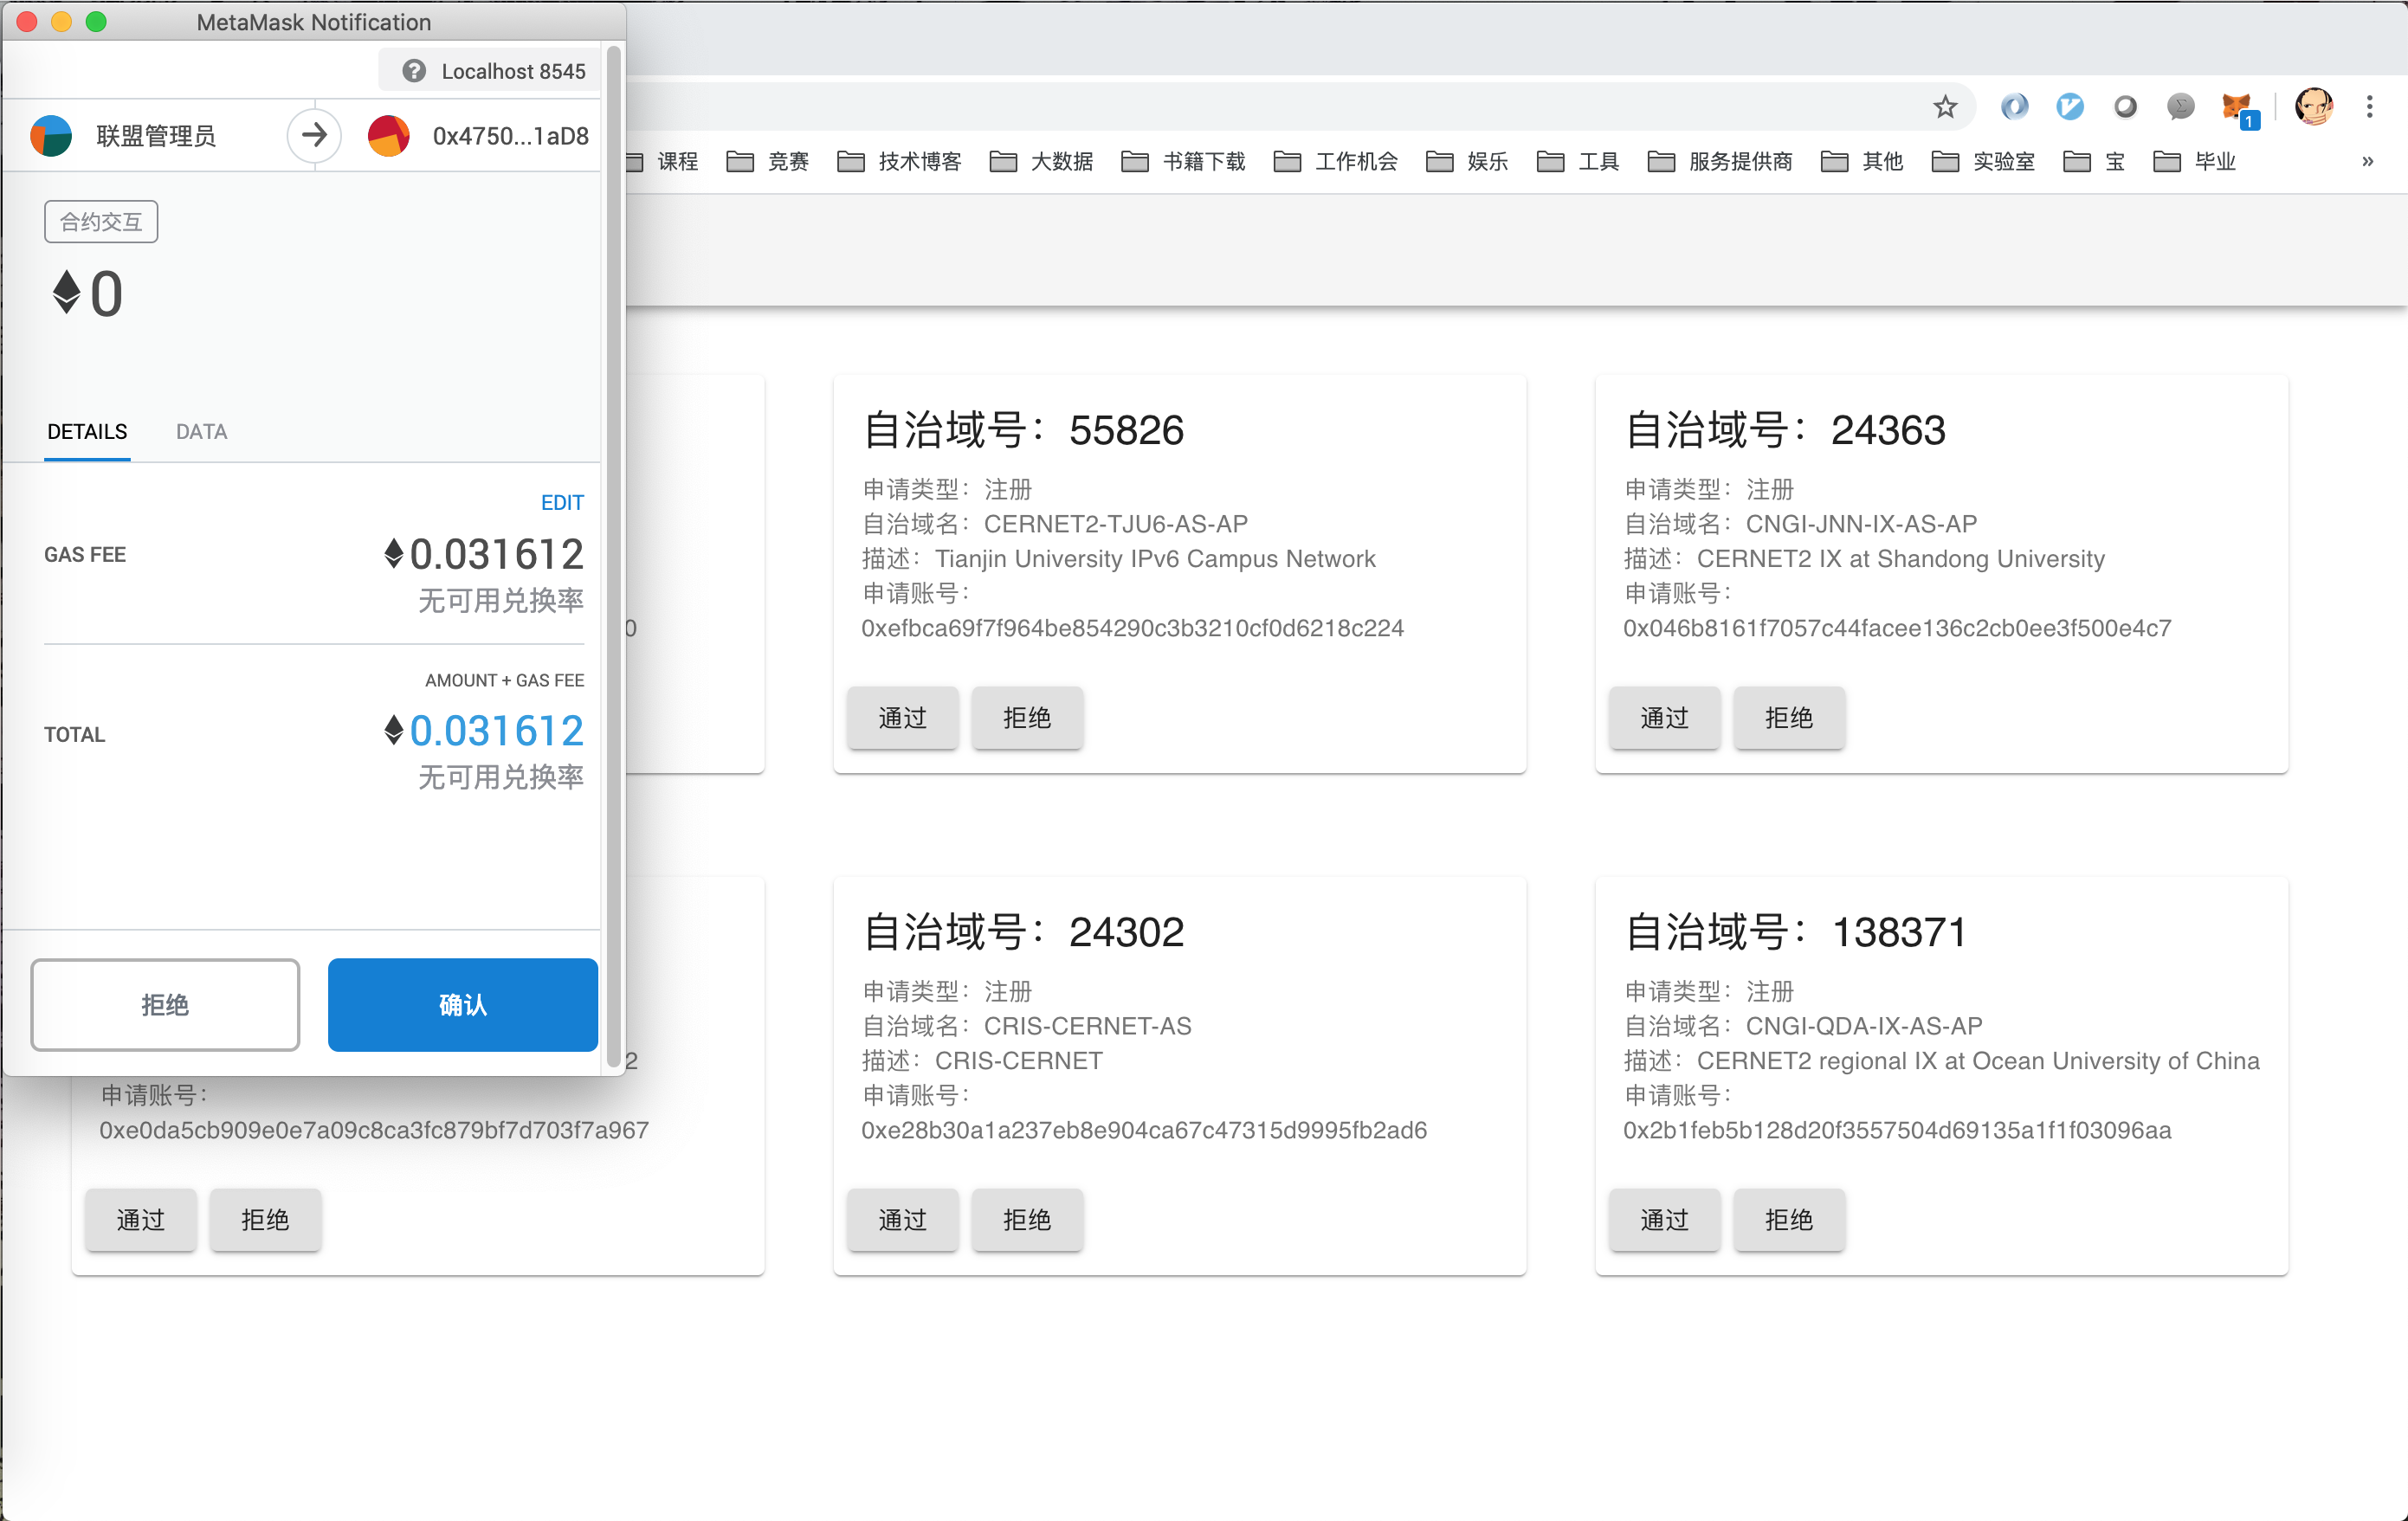
\includegraphics[height=4.5cm]{figures/regchain_client_review_1.png}}
        \hspace{1em}
        \subcaptionbox{非管理员无法审批\label{fig:regchain_client_review_2}}
        {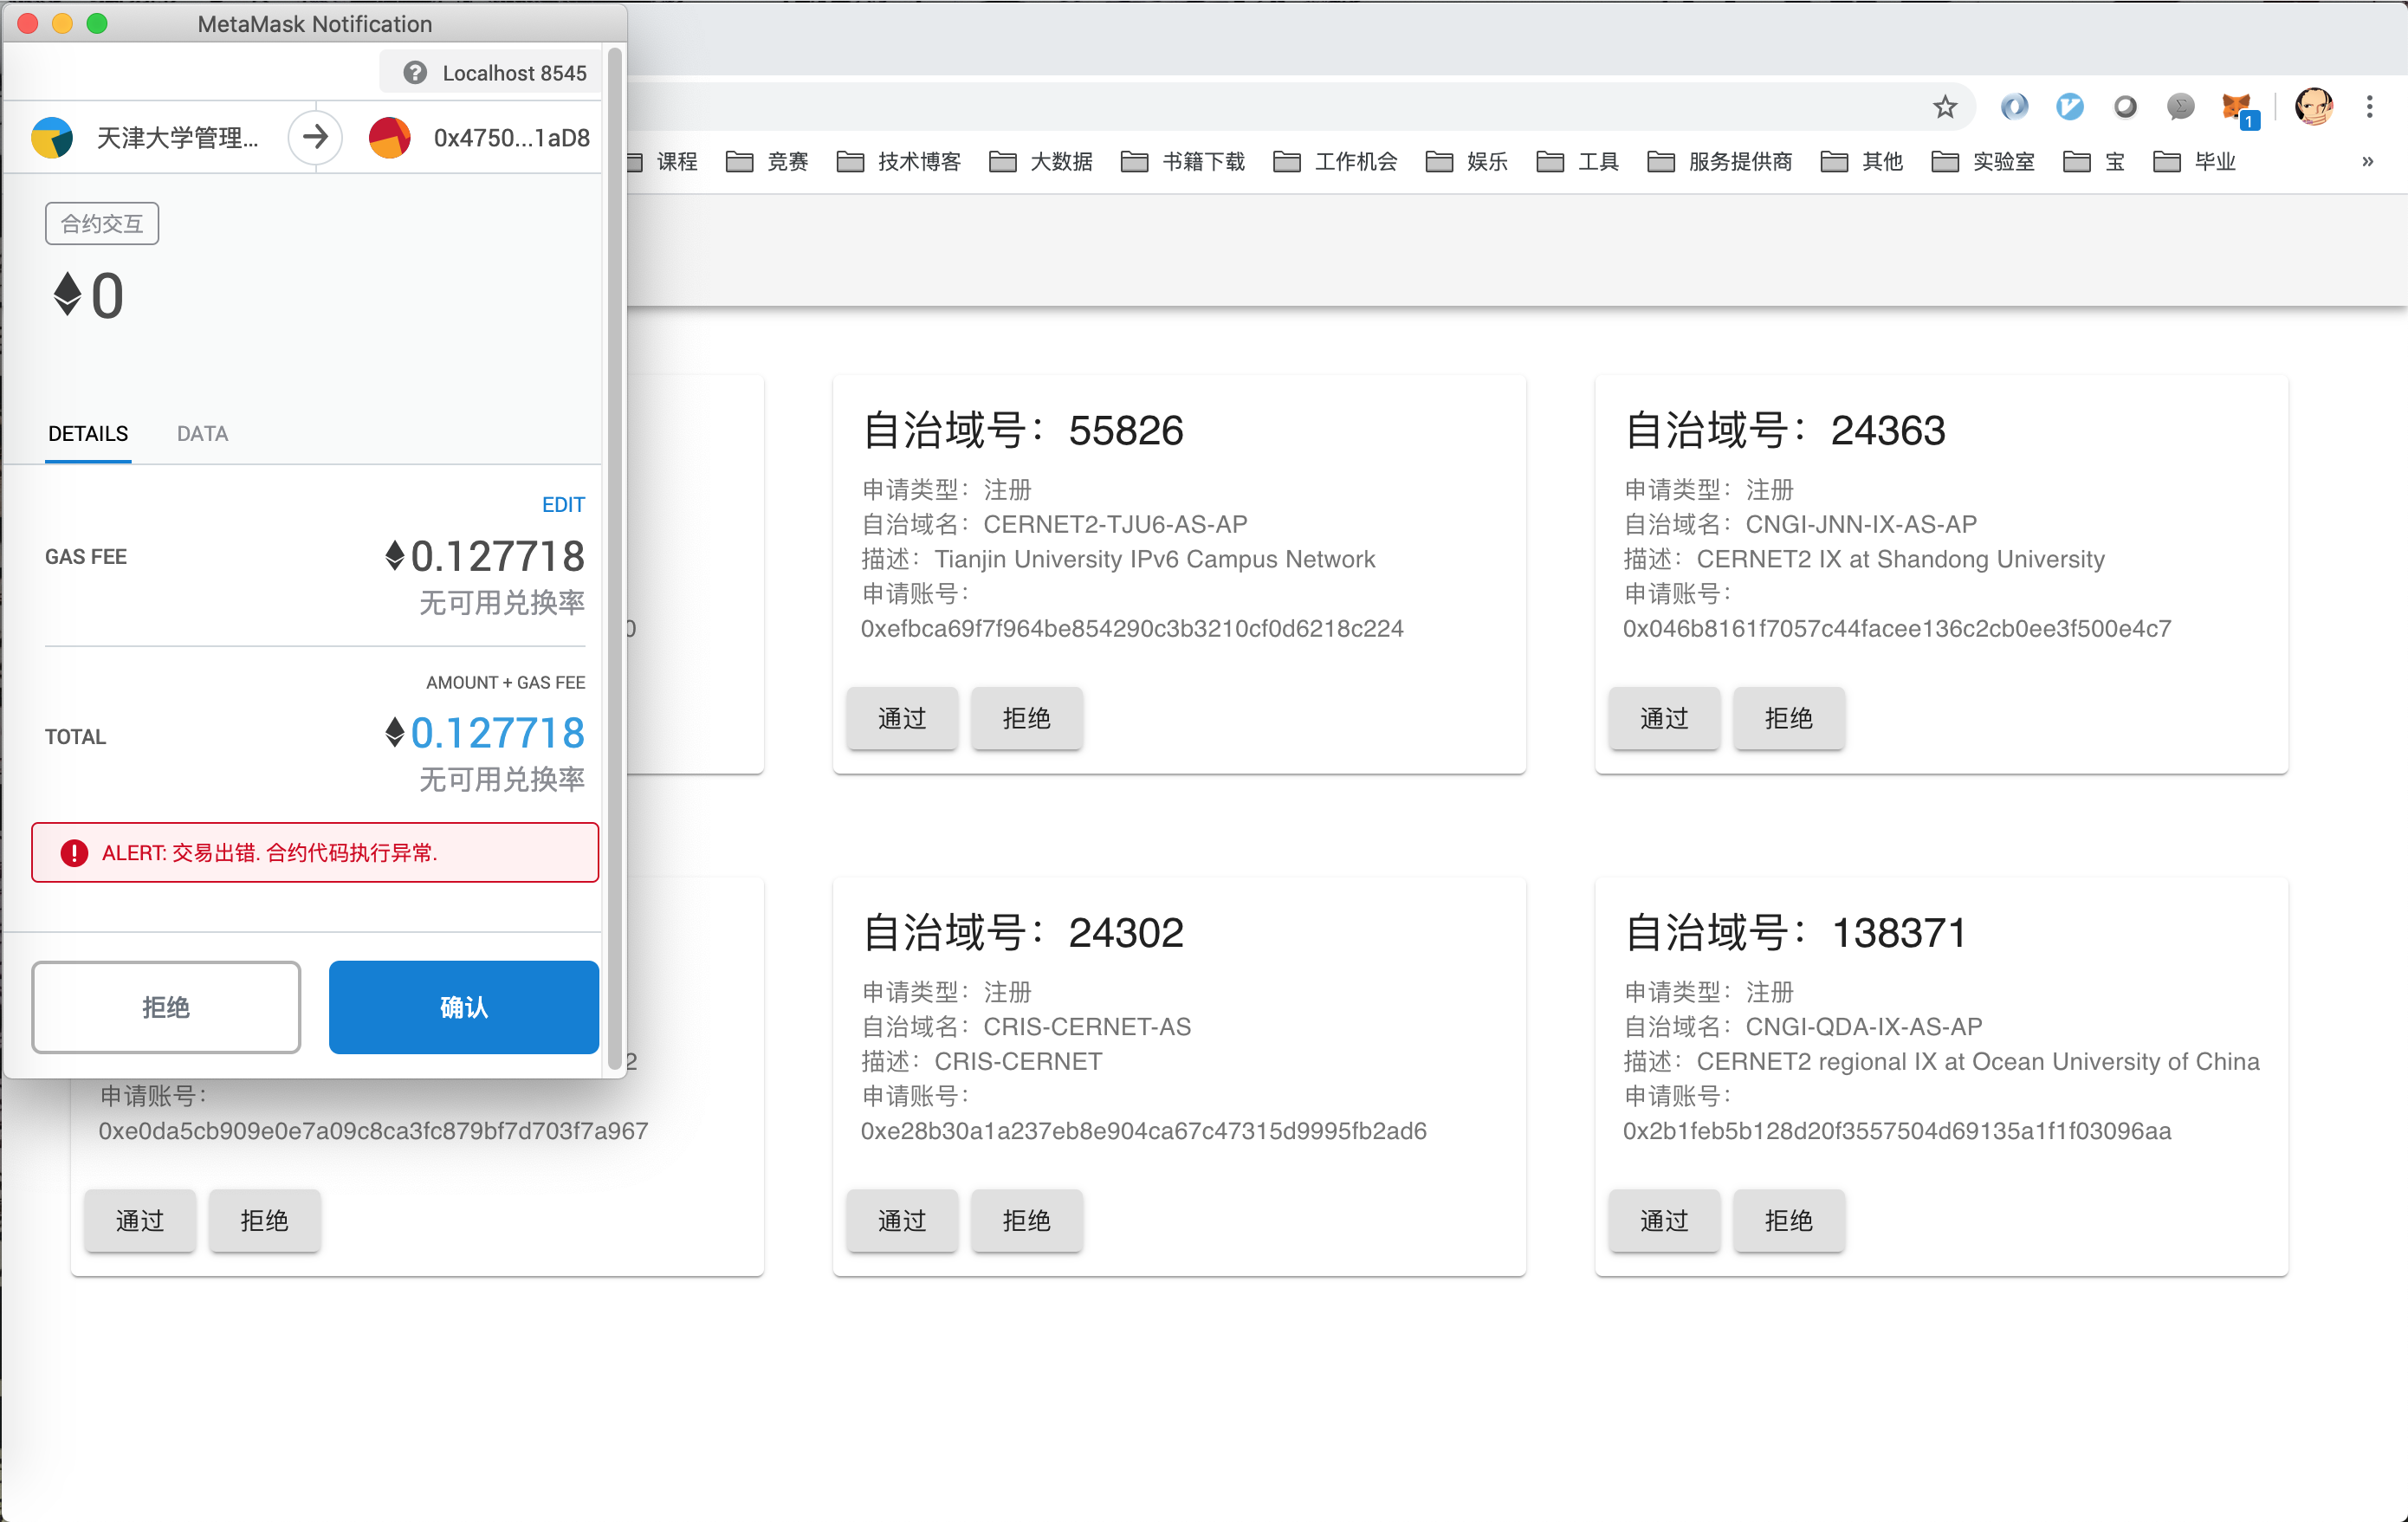
\includegraphics[height=4.5cm]{figures/regchain_client_review_2.png}}
        \caption{RegChain自治域审批页面}
        \label{fig:regchain_client_review}
      \end{figure}

      各个自治域管理员可通过“自治域查询”查看当前联盟内各个自治域的信息与当前有效的ACS地址。当点击自身管理的自治域显示卡时,将弹出窗口允许其对ACS信息进行配置,如图\ref{fig:regchain_client_update_1}所示。当点击其他自治域的显示卡时,也将弹出窗口显示具体信息,但不允许配置ACS信息,如图\ref{fig:regchain_client_update_2}所示,即使是联盟管理员也无法配置联盟内其他自治域的ACS地址。

      \begin{figure}[H]
        \centering
        \subcaptionbox{管理员正常更新\label{fig:regchain_client_update_1}}
        {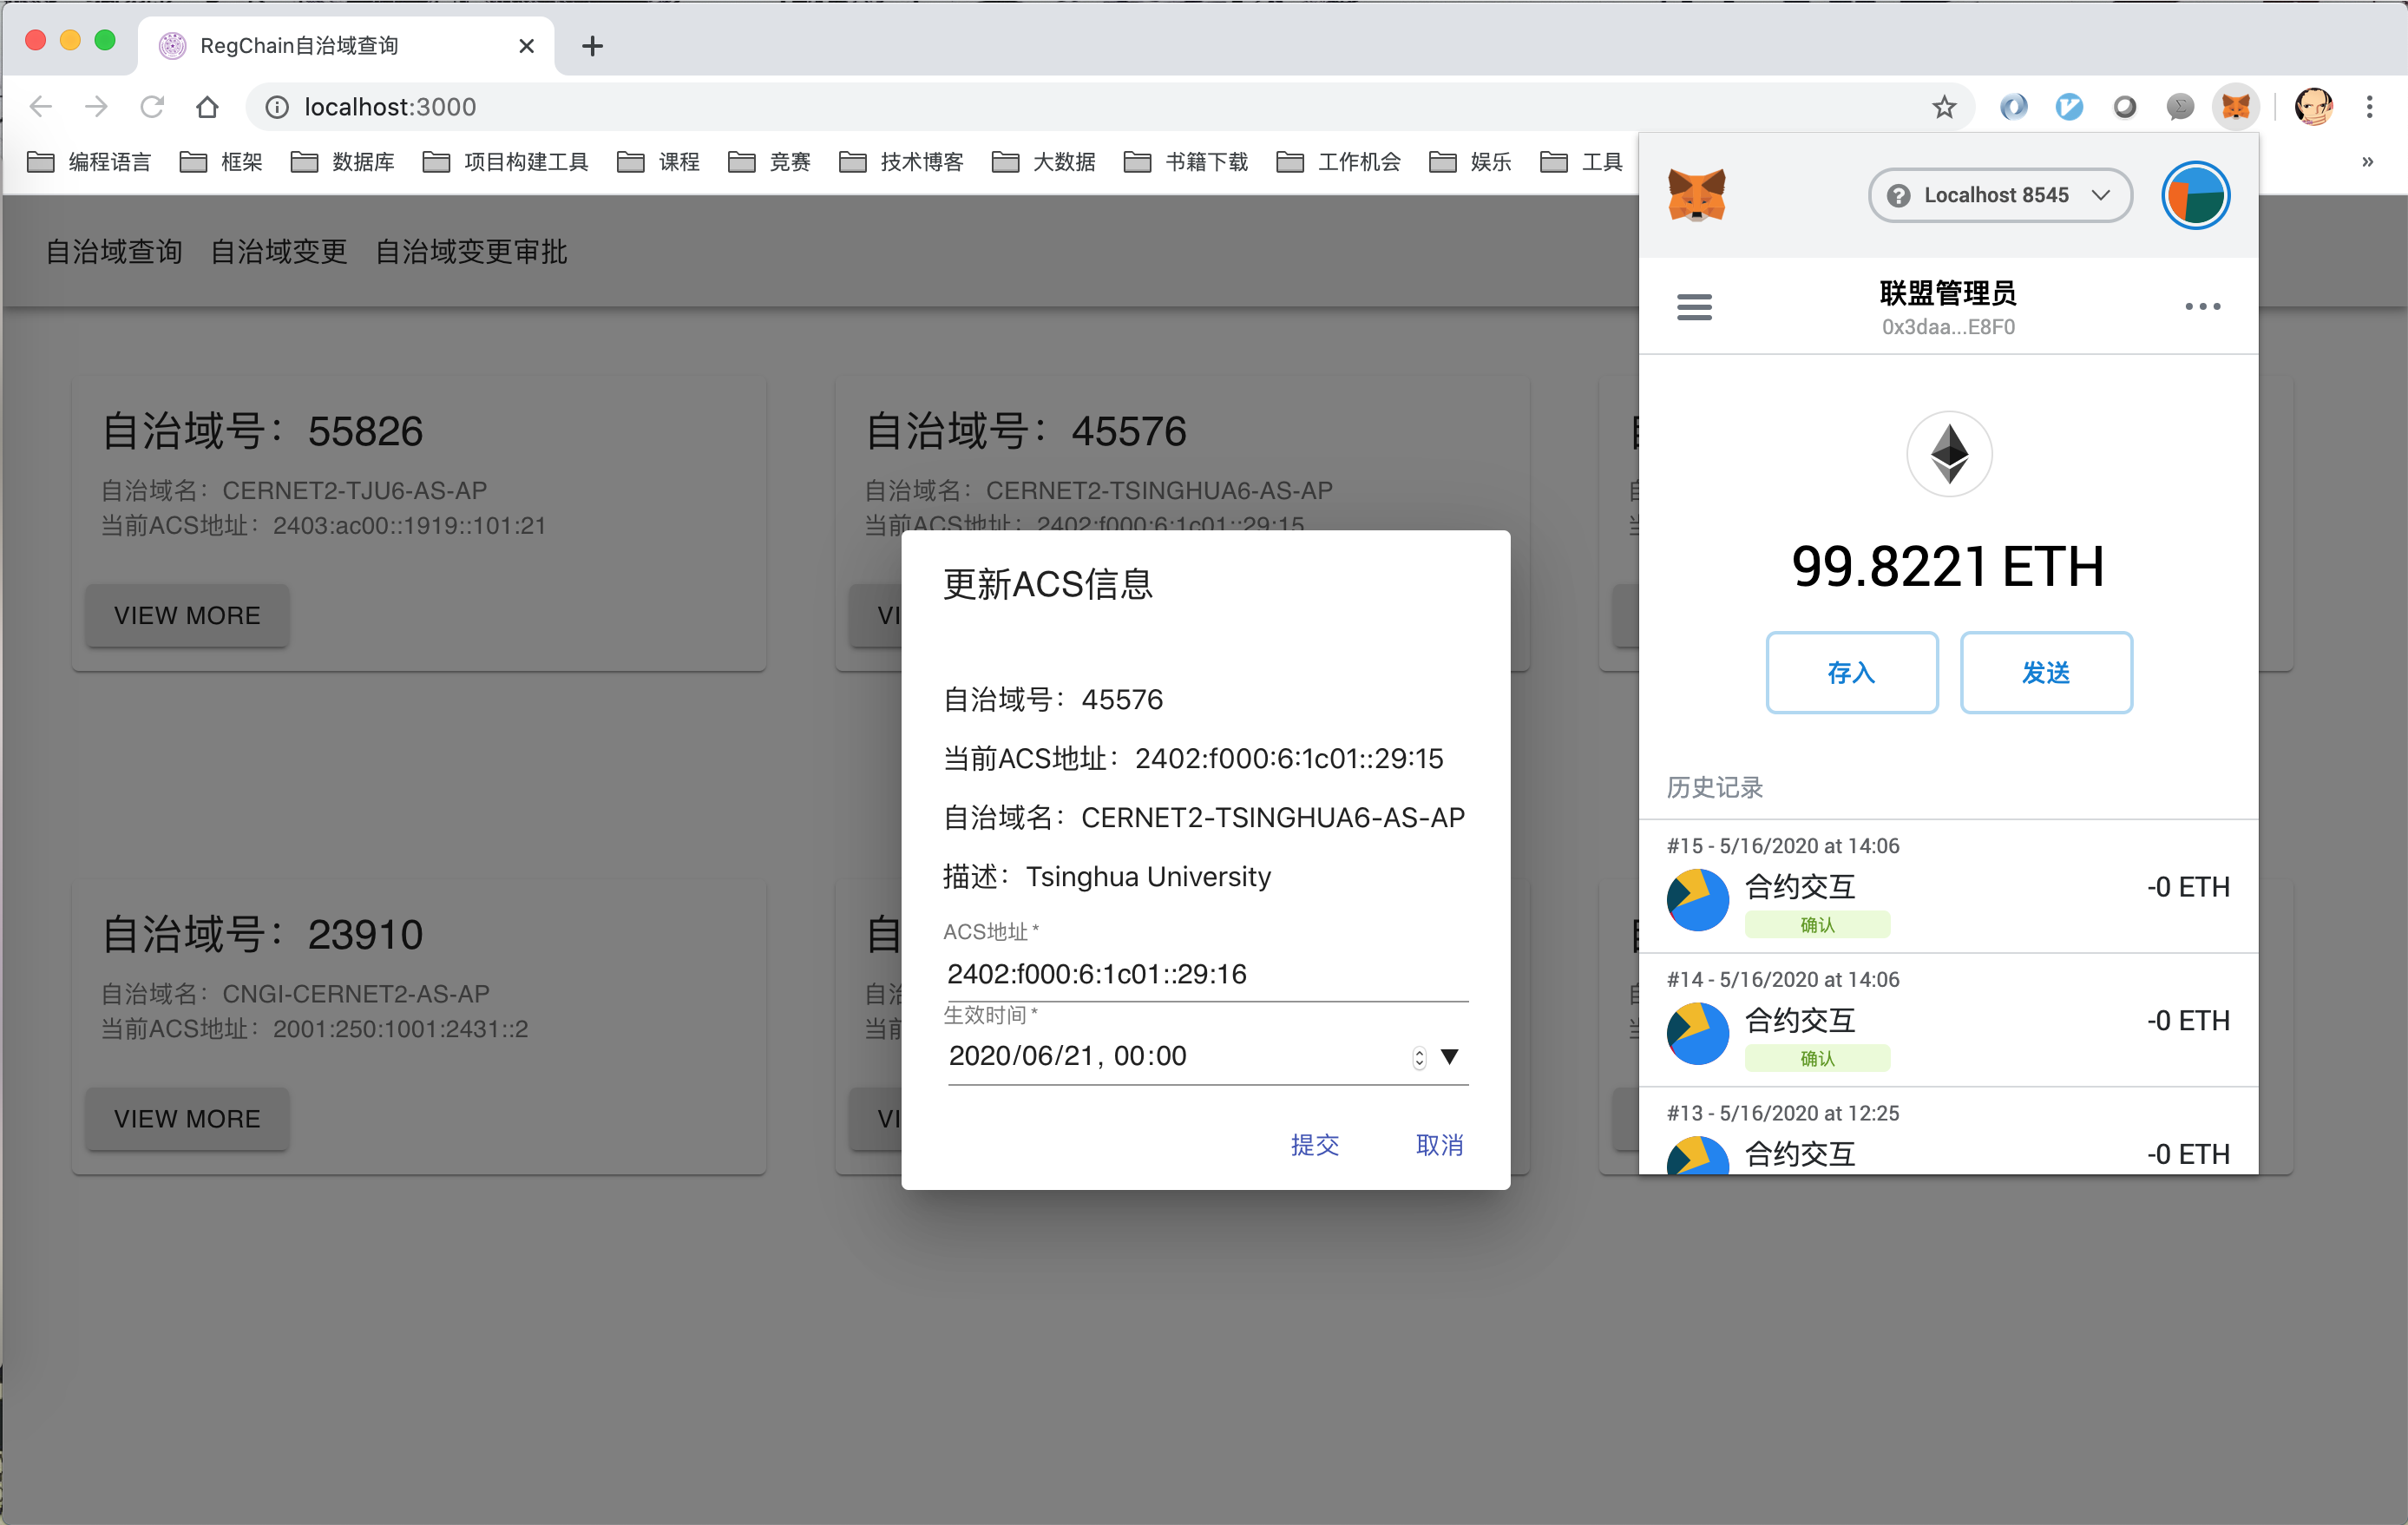
\includegraphics[height=4.5cm]{figures/regchain_client_update_1.png}}
        \hspace{1em}
        \subcaptionbox{非管理员无法更新\label{fig:regchain_client_update_2}}
        {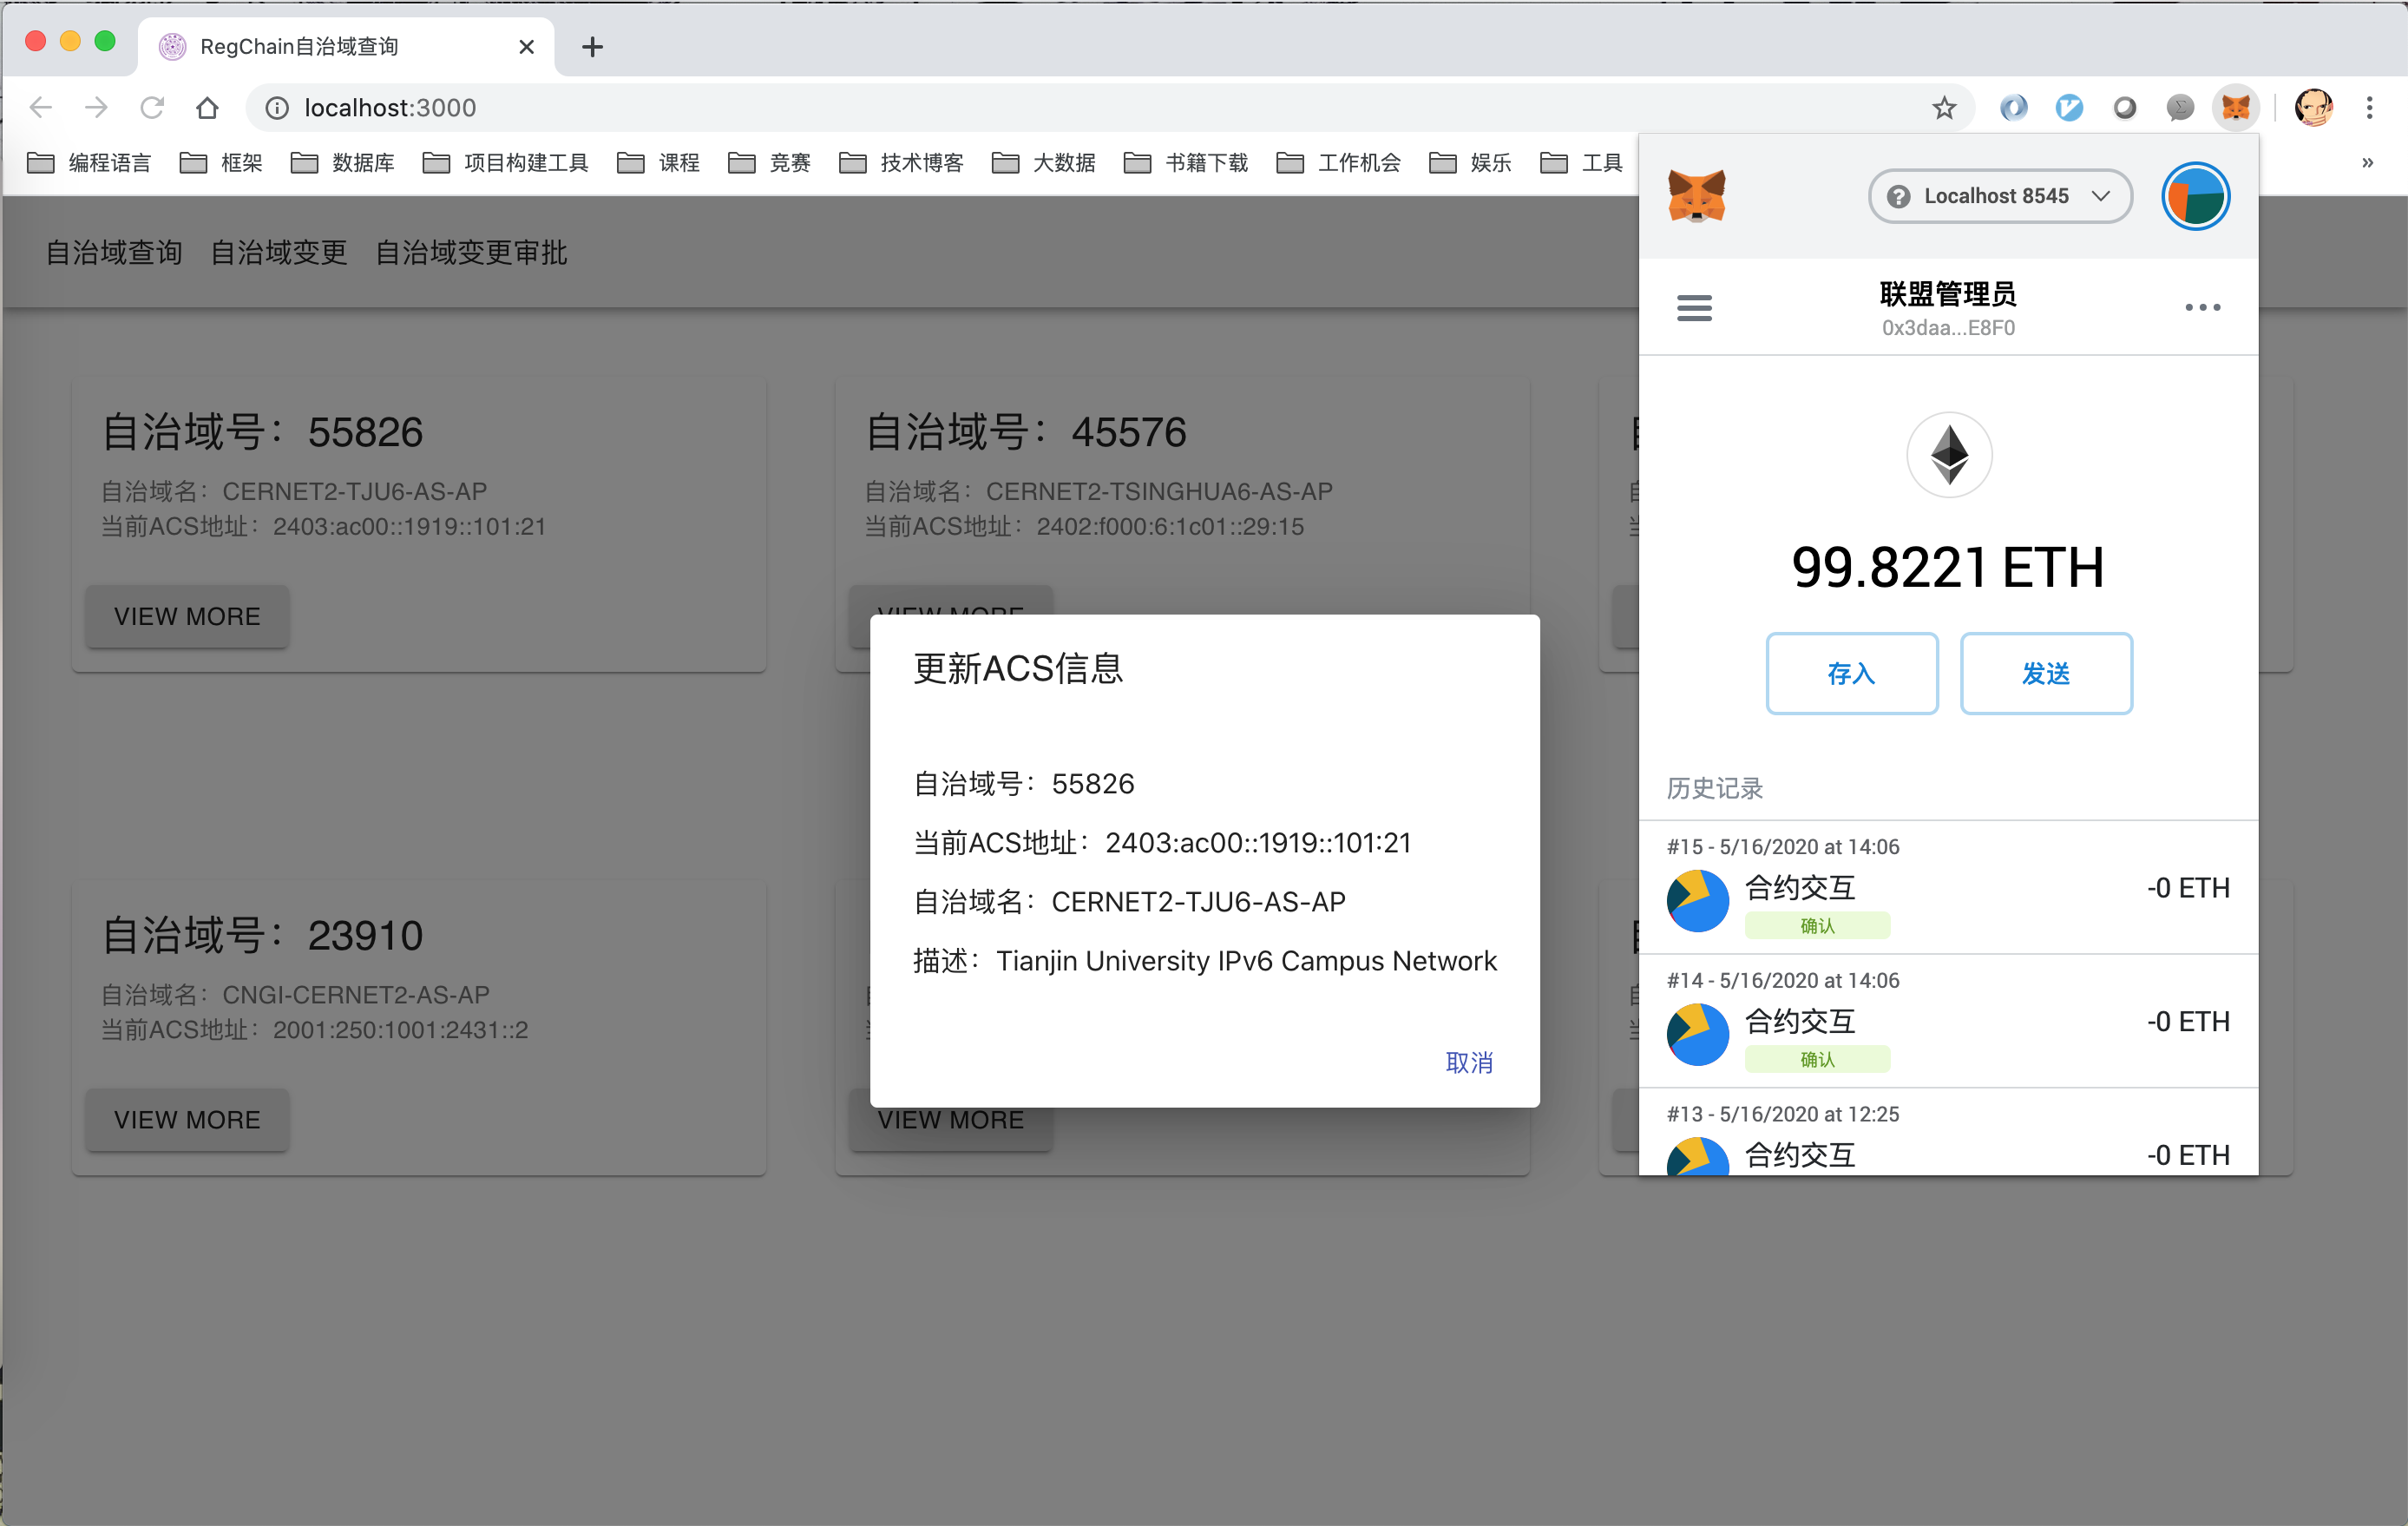
\includegraphics[height=4.5cm]{figures/regchain_client_update_2.png}}
        \caption{RegChain自治域ACS更新页面}
        \label{fig:regchain_client_update}
      \end{figure}

      自治域信息拉取服务的封装接口忽略了时间参数,其将自动根据系统时间计算当前时间进行参数填充,内部直接通过web3.js调用SMARegister.ASQuery与ASInfo.getCurrentACS获取联盟内所有自治域的当前ACS地址。

      \subsubsection{系统性能测试}
      \label{IPv6_Security:interas:implement:test}

      RegChain支持的各项操作由客户端与DApp两部分组成。自治域申请、审批操作在客户端仅需签发交易,在DApp侧则需要等待出块与合约执行。RegChain的出块速度与创建创世区块时设定的难度值相关,与RegChain的网络规模不相关,考虑到自治域信息更新操作要求的实时性不高,且并不频繁,本文在测试时将其难度值设定为0x4cccc8,以平均15秒的速度进行出块。

      本文以CNGI-CERNET2接入41所高校组成SMA安全联盟为例,采用41个区块链节点的网络规模对SMA联盟注册系统各项功能的性能进行了测试,结果如表\ref{tab:sma_ethereum_performance}所示。
      \begin{table}[htb]
        \centering
        \begin{minipage}[t]{\linewidth} 
          \caption{SMA联盟注册系统的以太坊实现性能测试}
          \label{tab:sma_ethereum_performance}
          \begin{tabularx}{\linewidth}{>{\centering\arraybackslash}X>{\centering\arraybackslash}X>{\centering\arraybackslash}X}
            \toprule[1.5pt]
            {\heiti 功能} & {\heiti 客户端时间(ms)} & {\heiti 合约时间(ms)} \\\midrule[1pt]
            {\heiti 自治域申请提交} & 8 & 69 \\
            {\heiti 自治域申请通过} & 7 & 69 \\ 
            {\heiti 自治域申请拒绝} & 7 & 50 \\ 
            {\heiti 自治域申请查询} & 6 & 131 \\ 
            {\heiti 单个ACS信息查询} & 7 & 13 \\ 
            {\heiti 全联盟ACS信息查询} & 7 & 71 \\ 
            \bottomrule[1.5pt]
          \end{tabularx}
        \end{minipage}
      \end{table}

      可见,由于各项操作在客户端处均为收集表单信息并发送交易,因此耗时基本相同。在DApp侧,自治域申请与审批操作由于需要向区块链中写入数据,因此耗时较多。自治域申请查询与ACS信息查询操作不需要更改区块链状态,但由于自治域数量较多,存在拷贝自治域信息的开销,因此尽管单个自治域查询时间极短,但进行全量查询时仍耗费了比自治域信息更新更多的时间。总而言之,各个操作均在远小于1秒的时间内完成,就用户体验而言拥有媲美单机服务器的性能。对于提交自治域更新或审批自治域更新请求等操作,至多等待15秒即可在区块链上看到相应数据的记录。

    \subsection{自治域间源地址验证技术安全性的进一步讨论}
    \label{IPv6_Security:interas:discuss}
    本文提出的RegChain方案主要针对自治域间源地址验证技术本身设计中的安全问题进行研究,其本质上是以一种避免数据篡改和降低服务不可用风险的分布式数据库替代了原本安全联盟采用的单点数据库,从而规避了因为联盟注册中心服务器的故障而导致整个联盟内跨自治域报文转发出现问题的风险,这种设计同样可以推广到其他所有基于安全联盟来建立自治域间信任关系的域间源地址验证方案中。对于其他的端到端类域间源地址验证方案,RegChain可根据其设计中安全联盟维护的信息对SMARegister与ASInfo的函数接口和内部数据结构进行相应的调整,从而适应不同格式的信息记录,为所有基于联盟的端到端类域间源地址验证技术提供统一的安全性提升方案。

    在SMA方案的设计中,各自治域持有的IPv6地址资源由自治域ACS之间建立通信协商状态机时进行公告,而非登记在RegChain中。尽管安全联盟机制能够保证一定程度的自治域间互信关系,但攻击者仍可能瞄准各自治域ACS发动攻击,篡改其宣告的IPv6地址以造成自治域间跨域报文转发的错误过滤等问题。RPKI\cite{RFC6480}可以提供对地址资源所有权的验证,从而解决宣告或使用虚假的IPv6地址的问题。但其同样面临单一故障点的困境,将其建设为区块链以分布式地记录地址资源所有权,可以进一步提升域间源地址验证技术的安全性,为用户身份识别与溯源系统提供更为牢固的IPv6地址真实性基础。

    本文所研究的RegChain方案属于论文作者所在实验室与华为网络技术实验室所合作的去中心化网络基础设施项目中的一部分,在该项目中还将研究利用区块链提升域间路由系统BGP\cite{RFC4271}、域名系统DNS\cite{RFC1034,RFC1035}等基础设施安全性的方案。

  \section{本章小结}
  \label{IPv6_Security:summary}
  本章从接入子网与自治域间两个层次的源地址验证技术分析出发,对SAVI技术在非理想网络环境中的部署问题与端到端类域间源地址验证技术的中心化风险分别提出了安全性增强的方案。主机粒度的源地址验证与跨自治域的源地址伪造预防是实现多组织用户身份识别与溯源技术的前提,这两者的增强方案的提出将进一步强化用户身份溯源机制带来的威慑能力。